\chapter{\label{chapterNumericalExperiments}Numerical experiments}

In this chapter, we are going to measure the performance of our algorithms by applying them to an example of the weak problem \eqref{weakProb}. For this purpose, the solution of this problem is derived first. Afterwards, we compare the analytical solution with the solution from the FOM-EnOpt and the Adaptive-ML-EnOpt (AML-EnOpt) algorithm. Additionally, we examine how the optimization algorithms behave if parameters, such as the number of time steps, are changed or if other neural network structures are used.

\section{Example of an analytical problem}

This section begins with a definition. We cite from \cite{articleMeidner} with a slightly different notation.

\begin{defn}[Directional derivative.]
Let $Y$ and $Z$ be normed vector spaces, $Y_0$ be a nonempty subset of $Y$ and $g:Y_0\to Z$ be a given mapping. If for two elements $y\in Y_0$ and $\delta_y\in Y$ the limit
\begin{displaymath}
g'(y)(\delta_y):=\lim_{\tau\downarrow0}\frac{g(y+\tau\delta_y)-g(y)}{\tau}
\end{displaymath}
exists, then $g'(y)(\delta_y)$ is called the directional derivative of $g$ at $y$ in direction $\delta_y$. If this limit exists for all $\delta_y\in Y$, then $g$ is called directionally differentiable at $y$.
\end{defn}
We now state a proposition about the directional derivative of $j$.
\begin{prop}
\label{jDirectionalDerivativeProp}
Let $j(q)=J(q,u(q))$ with $J$ as in \eqref{weakProb}. $j$ is directionally differentiable for all $q\in Q$. If a $z=z(q)\in X$ exists which satisfies the adjoined state equation
\begin{equation}
\label{adjoinedStateEquation}
\begin{aligned}
	-(\phi,\partial_tz)_I+(\nabla \phi,\nabla z)_I&=(\phi, u(q)-\hat{u})_I&\forall\phi\in X,\\
	z(T)&=0&\text{ in }\Omega,
\end{aligned}
\end{equation}
then $j$ has the directional derivative
\begin{equation*}
j'(q)(\delta_q)=(\alpha q+z(q),\delta_q)\text{ for all $\delta_q\in Q$}.
\end{equation*}
\end{prop}
\begin{proof}
If one does not know the adjoined state equations, the adjoined state method as it is applied in \cite{Plessix2006ARO} might help for the computation of the directional derivative. We calculate the directional derivative directly since it is already known to us by \cite{doi:10.1137/070694016}.

Let $q,\delta_q \in X$ and let $\delta_u\in X$ be defined so that it satisfies
\begin{equation}
\label{deltaUEquations}
\begin{aligned}
	(\partial_t\delta_u,\phi)_I+(\nabla \delta_u,\nabla\phi)_I&=(\delta_q,\phi)_I&\forall\phi\in X,\\
	\delta_u(0)&=0&\text{ in }\Omega.
\end{aligned}
\end{equation}
Such a solution exists uniquely by Proposition \ref{uniqueU}. Now it holds, that for any $\tau\in\mathbb{R}$,
\begin{equation*}
\begin{aligned}
	(\partial_t(u(q)+\tau\delta_u),\phi)_I+(\nabla (u(q)+\tau\delta_u),\nabla\phi)_I&=(f+q+\tau\delta_q,\phi)_I&\forall\phi\in X,\\
	(u(q)+\tau\delta_u)(0)&=u_0&\text{ in }\Omega
\end{aligned}
\end{equation*}
by multplication of the equations in \eqref{deltaUEquations} with $\tau$ and addition of the product to the weak state equations \eqref{weakEq}. Since $u(q+\tau\delta_q)$ is uniquely defined to satisfy the equations
\begin{equation}
\label{partialDerivativeInDeltaUDir}
\begin{aligned}
	(\partial_tu(q+\tau\delta_q),\phi)_I+(\nabla u(q+\tau\delta_q),\nabla\phi)_I&=(f+q+\tau\delta_q,\phi)_I&\forall\phi\in X,\\
	u(q+\tau\delta_q)(0)&=u_0&\text{ in }\Omega,
\end{aligned}
\end{equation}
it follows that $u(q+\tau\delta_q)=u(q)+\tau\delta_u$. By using this, we calculate

\begin{eqnarray*}
&\lim_{\tau\downarrow0}&\frac{j(q+\tau\delta_q)-j(q)}{\tau}\\
=&\lim_{\tau\downarrow0}&\frac{1}{2\tau}\left(\|u(q+\tau\delta_q)-\hat{u}\|^2_I-\|u(q)-\hat{u}\|^2_I\right)\\
&&+\frac{\alpha}{2\tau}\left(\|q+\tau\delta_q\|^2_I-\|q\|^2_I\right)\\
=&\lim_{\tau\downarrow0}&\frac{1}{2\tau}\left(\|u(q)+\tau\delta_u-\hat{u}\|^2_I-\|u(q)-\hat{u}\|^2_I\right)\\
&&+\frac{\alpha}{2\tau}\left(\|q+\tau\delta_q\|^2_I-\|q\|^2_I\right).
\end{eqnarray*}
From $\|q+\tau\delta_q\|^2_I=\|q\|^2_I+2\tau(\delta_q,q)_I+\tau^2\|\delta_q\|^2_I$ follows that this term is equal to
\begin{eqnarray*}
&&\lim_{\tau\downarrow0}\frac{1}{2\tau}\left(2\tau(\delta_u,u(q)-\hat{u})_I+\tau^2\|\delta_u\|^2_I+\alpha\left(2\tau(\delta_q,q)_I+\tau^2\|\delta_q\|^2_I\right)\right)\\
&=&(\delta_u,u(q)-\hat{u})_I+\alpha(\delta_q,q)_I\\
&=&j'(q)(\delta_q)
\end{eqnarray*}

Let $u=u(q)$. By the first equation in \eqref{adjoinedStateEquation}, it holds

\begin{equation*}
(\delta_u,u-\hat{u})_I=-(\delta_u,\partial_tz)_I+(\nabla\delta_u,\nabla z)_I.
\end{equation*}
Integration by parts gives us
\begin{equation*}
(\delta_u,u-\hat{u})_I=-(\delta_u(T),z(T))+(\delta_u(0),z(0))+(\partial_t\delta_u,z)_I+(\nabla\delta_u,\nabla z)_I.
\end{equation*}
From $z(T)=0\text{ in }\Omega$ from \eqref{adjoinedStateEquation} and $\delta_u(0)=0\text{ in }\Omega$ from \eqref{deltaUEquations} follows
\begin{equation*}
(\delta_u,u-\hat{u})_I=(\partial_t\delta_u,z)_I+(\nabla\delta_u,\nabla z)_I.
\end{equation*}
Applying the first equation from \eqref{deltaUEquations} yields
\begin{equation*}
(\delta_u,u-\hat{u})_I=(\delta_q,z)_I.
\end{equation*}
Now we conclude
\begin{equation*}
j'(q)(\delta_q)=(\alpha q+z(q),\delta_q).
\end{equation*}
\end{proof}

We now want to find a stationary point $\bar{q}$ of $j$ such that
\begin{equation}
\label{firstOrderOptimalityCondition}
j'(\bar{q})(\delta_q)=0\quad\forall \delta_q\in Q.
\end{equation}
If \eqref{firstOrderOptimalityCondition} holds, then $\bar{q}$ satisfies the first order optimality conditions of \eqref{redProb}. In this case, $\bar{q}$ is even optimal due to the linear-quadratic structure of the optimal control problem \cite{doi:10.1137/070694016}.\\

For the testing of our algorithms, we consider the problem \eqref{weakProb} on $\Omega\times I=(0,1)^2\times(0,T)$ with $T=0.1$. The following example is originally described in \cite{doi:10.1137/070694016}. To define the functions in \eqref{weakProb}, we use the eigenfunction
\begin{displaymath}
w_a(t,x_1,x_2):=\exp(a\pi^2t)\sin(\pi x_1)\sin(\pi x_2) \text{ for } a\in\mathbb{R}.
\end{displaymath}

Now we set

\begin{equation}
\label{exampleProblemDefinitions}
\begin{aligned}
f(t,x_1,x_2)\quad:=\quad&-\pi^4w_a(T,x_1,x_2),&\\
\hat{u}(t,x_1,x_2)\quad:=\quad&\frac{a^2-5}{2+a}\pi^2w_a(t,x_1,x_2)+2\pi^2w_a(T,x_1,x_2),&\\
u_0(x_1,x_2)\quad:=\quad&\frac{-1}{2+a}\pi^2w_a(0,x_1,x_2).&
\end{aligned}
\end{equation}

The next proposition states the optimal solution of the problem that is described above.
\begin{prop}
If we set the regularization parameter $\alpha$ in the objective functional \eqref{objFun} as $\pi^{-4}$, we get the optimal solution $(\bar{q}, \bar{u}, \bar{z})$ of the problem \eqref{weakProb} on $\Omega\times I=(0,1)^2\times(0,T)$ with $T=0.1$ and the functions from \ref{exampleProblemDefinitions}, where
\begin{equation}
\label{analyticalSolution}
\begin{aligned}
\bar{q}(t,x_1,x_2)\quad:=\quad&-\pi^4\left(w_a(t,x_1,x_2)-w_a(T,x_1,x_2)\right),&\\
\bar{u}(t,x_1,x_2)\quad:=\quad&\frac{-1}{2+a}\pi^2w_a(t,x_1,x_2),&\\
\bar{z}(t,x_1,x_2)\quad:=\quad&w_a(t,x_1,x_2)-w_a(T,x_1,x_2).&
\end{aligned}
\end{equation}
\end{prop}
\begin{proof}
It holds that $\bar{q}\in Q, \bar{u}\in X, \bar{z}\in X$. We confirm now that $(\bar{q}, \bar{u}, \bar{z})$ is a minimizer by checking if $\bar{q}$ satisfies \eqref{firstOrderOptimalityCondition}, $\bar{u}$ \eqref{weakEq} and $\bar{z}$ \eqref{adjoinedStateEquation}.

Beginning with $\bar{z}$, we have $\bar{z}(T, x_1, x_2)=0$ trivially for all $(x_1,x_2)\in\Omega$ and therefore the second equation in \eqref{adjoinedStateEquation} is satisfied. To check the first equation in \eqref{adjoinedStateEquation}, we write it as
\begin{displaymath}
(\phi,\partial_tz)_I-(\nabla \phi,\nabla z)_I+(\phi, u-\hat{u})_I=0\quad\forall\phi\in X.
\end{displaymath}
Integration by parts gives for all $\phi\in X$
\begin{displaymath}
(\phi,\partial_tz)_I-(\nabla \phi,\nabla z)_I+(\phi, u-\hat{u})_I=(\phi,\partial_tz+\Delta z+u-\hat{u})_I.
\end{displaymath}
Now we compute
\begin{eqnarray*}
\partial_t\bar{z}(t,x_1,x_2)&=&\partial_tw_a(t,x_1,x_2)\\
&=&a\pi^2w_a(t,x_1,x_2)\\
\Delta \bar{z}(t,x_1,x_2)&=&2\pi^2(w_a(T,x_1,x_2)-w_a(t,x_1,x_2))\\
\bar{u}(t,x_1,x_2)-\hat{u}(t,x_1,x_2)&=&\pi^2((2-a)w_a(t,x_1,x_2)-2w_a(T,x_1,x_2)).
\end{eqnarray*}
From $\partial_t\bar{z}(t,x_1,x_2)+\Delta \bar{z}(t,x_1,x_2)+\bar{u}(t,x_1,x_2)-\hat{u}(t,x_1,x_2)=0$ for all $(x_1,x_2)\in\Omega, t\in I$ follows now that $\bar{z}$ satisfies the adjoined state equation \eqref{adjoinedStateEquation}.

By doing the same for $\bar{u}$, we see that it meets the initial condition $\bar{u}(0,x_1,x_2)=u_0(x_1,x_2)$ for all $(x_1,x_2)\in\Omega$ of \eqref{weakEq}. Again, we write the first equation in \eqref{weakEq} as
\begin{displaymath}
(\partial_tu,\phi)_I+(\nabla u,\nabla\phi)_I-(f+q,\phi)_I=0\quad\forall\phi\in X,
\end{displaymath}
and integration by parts gives us for all $\phi\in X$
\begin{displaymath}
(\partial_t\bar{u},\phi)_I+(\nabla \bar{u},\nabla\phi)_I-(f+\bar{q},\phi)_I=(\partial_t\bar{u}-\Delta\bar{u}-f-\bar{q},\phi)_I.
\end{displaymath}
It holds
\begin{eqnarray*}
\partial_t\bar{u}(t,x_1,x_2)&=&\frac{-a}{2+a}\pi^4w_a(t,x_1,x_2)\\
\Delta \bar{u}(t,x_1,x_2)&=&\frac{2}{2+a}\pi^4w_a(t,x_1,x_2)\\
\partial_t\bar{u}(t,x_1,x_2)-\Delta \bar{u}(t,x_1,x_2)&=&-\pi^4w_a(t,x_1,x_2)\\
&=&f(t,x_1,x_2)+\bar{q}(t,x_1,x_2).
\end{eqnarray*}
Therefore $\partial_t\bar{u}(t,x_1,x_2)-\Delta\bar{u}(t,x_1,x_2)-f(t,x_1,x_2)-\bar{q}(t,x_1,x_2)=0$ for all $(x_1,x_2)\in\Omega, t\in I$, so $\bar{u}$ fulfills the conditions of the weak state equation \eqref{weakEq}.

With $\alpha=\pi^{-4}$ we get $\alpha\bar{q}(t,x_1,x_2)+\bar{z}(t,x_1,x_2)=0$ for all $(x_1,x_2)\in\Omega, t\in I$, which means that $\bar{q}$ satisfies the optimality condition \eqref{firstOrderOptimalityCondition}. Now we conclude that $(\bar{q}, \bar{u}, \bar{z})$ is the optimal solution.
\end{proof}

Since the solutions $q\in Q_d$ of our algorithms have the form that is described in \eqref{discrContrVar}, we need to define a control-shape functional before we search for an optimizer. $\bar{q}$ can be written as
\begin{displaymath}
\bar{q}(t,x_1,x_2)=-\pi^4(\exp(a\pi^2t)-\exp(a\pi^2T))\sin(\pi x_1)\sin(\pi x_2).
\end{displaymath}
Now we have $\bar{q}$ as a product of the term $-\pi^4(\exp(a\pi^2t)-\exp(a\pi^2T))$, that is only dependent on $t$, and the shape functional $\sin(\pi x_1)\sin(\pi x_2)$, which depends only on $x$ and is an element of $H$. Additional shape functionals for the control functional are not used so that we can compare the outputs of our optimization algorithms with the analytical solution $\bar{q}$. We expect that the elements $q^i_1$ of the control vectors $\mathbf{q}$ that we get as outputs are close to
\begin{equation}
\label{controlVectorElements}
\bar{q}^i_1=-\pi^4(\exp(a\pi^2t_i)-\exp(a\pi^2T))\text{ for }i=0,\dotsc,N_t.
\end{equation}
For our tests, we choose $a$ to be $-\sqrt{5}$ which has the consequence that $f$ and $\hat{u}$ do not depend on time.

\section{Numerical results}

We now test the FOM- and AML-EnOpt algorithms on the example from the last section. For this, the space $\Omega=(0,1)^2$ is discretized as described in subsection \ref{SubsectionDiscretizationInSpace} with $50$ grid intervals. The time interval $I=(0,T)$ with $T=0.1$ that we observe is divided into $10$ smaller intervals which are all of the same size. This is described in subsection \ref{SubsectionDiscretizationInTime} with $N_t=10$. Since we have only one shape functional, the control vectors $\mathbf{q}$ that we search for have $N_\mathbf{q}=11$ elements. The resulting analytical control vector with elements as in \eqref{controlVectorElements} is depicted in Figure \ref{AnalyticalControlVectorPlot}. Its FOM objective functional value is approximately $4.2299573$. If we describe results in this chapter and nothing else is specified, we use the parameters given below.\\

\begin{figure}
\centering
%\textbf{Your title}\par\medskip
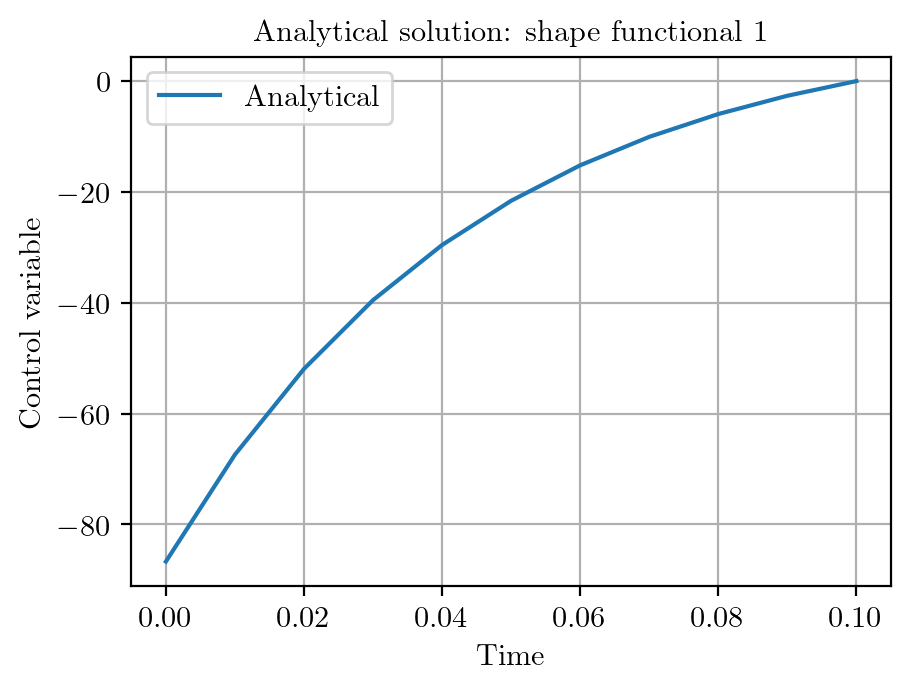
\includegraphics{Plots/analyticalControlVector.png}
\caption{\label{AnalyticalControlVectorPlot}The analytical control vector with elements $\bar{q}^i_1$ for $i=0,\dotsc,N_t$ as in \eqref{controlVectorElements}}
\end{figure}

The initial control vector $\mathbf{q}_0$ is a vector with constant entries of the value $-40$. This value lies approximately between the minimum element in \eqref{controlVectorElements} which is $\bar{q}^0_1\approx-87$ and the maximum $\bar{q}^{N_t}_1=0$. The values of the constant initial control vector, along with other parameters for the algorithms that are presented in the chapters \ref{ChapterEnsembleBasedOptimizationAlgorithm} and \ref{ChapterAdaptiveMLEnOptAlgorithm}, are specified in the Table \ref{FOMAMLEnOptParameters}. The notation in this table corresponds to the notation in these algorithms. We choose $\varepsilon_i$ to be smaller than $\varepsilon_o$ because an increase of inner optimization loops has only a small contribution to the computation time while it might lower the number of the more expensive outer iterations.

The neural network that is used for the surrogate functional consists of two hidden layers, where each hidden layer has $25$ neurons. Our activation function is the $\tanh$ function as mentioned in section \ref{sectionDeepNeuralNetworks}. Early stopping is applied for the training of the DNN with a maximum of $1000$ training epochs. The variable $\mathrm{earlyStop}$ in Algorithm \ref{trainDNN} is set to $15$. We use the L-BFGS optimizer with strong Wolfe line-search for the minimization of the MSE loss on the validation set. The learning rate of this optimizer is set to $10^{-2}$. The validation set consists of $20\%$ of the sample set, so the other $80\%$ of the sample set are used for the training set. Therefore, $\mathrm{trainFrac}$ in Algorithm \ref{DNNConstruction} is set to $0.8$. The number of training restarts is very small because a higher number would extend the training time of the DNN by so much that it makes the algorthm terminate slower. We restart the training two times, so we train three DNNs in total to construct the surrogate functional.\\

Before the results are presented, we want to note that the FOM-EnOpt and the Adaptive-ML-EnOpt procedures minimize the objective functional $j$ by maximizing the negative functional $-j$. The results that we show are converted back to the outputs that the objective functional $j$ would give, although the true values during the execution of these algorithms are negative. As an example, the graphs in Figure \ref{FOMAMLEnOptFuncValComp} would be mirrored on the $x$-axis if they had shown the values during the respective procedure.

Also, we want to clarify what we consider an outer and inner iteration. If we talk about the FOM-EnOpt algorithm, outer iterations involve computations of FOM optimization steps. Outer iterations in the FOM-EnOpt Algorithm \ref{EnOptAlg} are the first OptStep call in line \ref{EnOptAlgOptStepCall1} and passes of the while-loop from line \ref{EnOptAlgBeginWhile} to \ref{EnOptAlgEndWhile}. The first optimization step in line \ref{EnOptAlgOptStepCall1} is also considered an outer iteration because it has almost the same computational complexity as the calculations in the while-loop. Moreover, it changes the iterate. Inner iterations do not exist in this algorithm. In the AML-EnOpt algorithm, outer iterations include not only FOM optimization steps, but also the construction of a surrogate functional, and are therefore more expensive than the outer iterations of the FOM-EnOpt algorithm. In the Adaptive-ML-EnOpt Algorithm \ref{AML-EnOpt}, the computations from line \ref{F_k_tilde_check} to line \ref{AMLEnOptWhileEnd} are summed up as one outer iteration. The call of the FOM optimization step in line \ref{FOMOptStepAML1} is not considered an outer iteration loop because it is not as expensive as the computations in the outer iteration loop and also does not change the iterate during its call. Inner iterations are calls of the EnOpt algorithm on the neural network-based surrogate functional which occurs in line \ref{innerIterationCallAlgo} of the AML-EnOpt algorithm.

For consistency, we will refer during our explanations in this chapter to $\mathbf{q}_k$ as the iterate at the beginning of the outer iteration $k$ and $\mathbf{q}^\mathrm{next}_k$ as the iterate at the end of the outer iteration $k$. This is based on the notation of the AML-EnOpt Algorithm \ref{AML-EnOpt}. If we talk about the FOM-EnOpt algorithm, we refer to $\mathbf{q}_k$ as the iterate before the call of the optimization step procedure in line \ref{EnOptAlgOptStepCall1}, respectively line \ref{EnOptAlgOptStepCall2}, in the $k$-th outer iteration of the Algorithm \ref{EnOptAlg} and thus we denote $\mathbf{q}^\mathrm{next}_k$ as the iterate after this call in iteration $k$. Although, such a $\mathbf{q}^\mathrm{next}_k$ is not defined in the FOM-EnOpt algorithm.

\begin{table}
%\footnotesize
\caption{\label{FOMAMLEnOptParameters}Parameters used in the FOM-EnOpt and AML-EnOpt algorithms}
\centering
\begin{tabular}{ll}
\hline
Parameter & Value\\
\hline
Elements of the initial constant control vector $\mathbf{q}_0$ & -40\\
Initial step size $\beta_1$ & $1$\\
Initial covariance matrix adaption step size $\beta_2$ & $0.1$\\
Initial trust-region step size $\delta_\mathrm{init}$ & $100$\\
Step size contraction $r$ & $0.5$\\
Maximum step size trials $\nu^*$ & $10$\\
Maximum (outer/ inner) iterations $k^*, k^*_o, k^*_i$ & $1000$\\
Maximum trust-region iterations $k^*_\mathrm{TR}$ & $5$\\
Initial control variance $\sigma^2_1$ & $0.1$\\
Constant correlation factor $\rho$ & $0.9$\\
Sample size $N$ & $100$\\
FOM-EnOpt $\varepsilon$ & $10^{-8}$\\
Adaptive-ML-EnOpt inner iteration $\varepsilon_i$ & $10^{-12}$\\
Adaptive-ML-EnOpt outer iteration $\varepsilon_o$ & $10^{-8}$\\
%& $$\\
\hline
\end{tabular}
\end{table}

Figure \ref{FOMAMLEnOptFuncValComp} shows the development of the FOM objective functional value $j(\mathbf{q}^\mathrm{next}_k)$ after each outer iteration during the FOM- and AML-EnOpt procedures, as well as the respective functional value $j^k_\mathrm{ML}(\mathbf{q}^\mathrm{next}_k)$ of the surrogate functional $j_\mathrm{ML}^k$ that is used in line \ref{innerIterationCallAlgo} of the AML-EnOpt Algorithm \ref{AML-EnOpt} to compute the iterate $\mathbf{q}^\mathrm{next}_k$.

\begin{figure}
\centering
%\textbf{Your title}\par\medskip
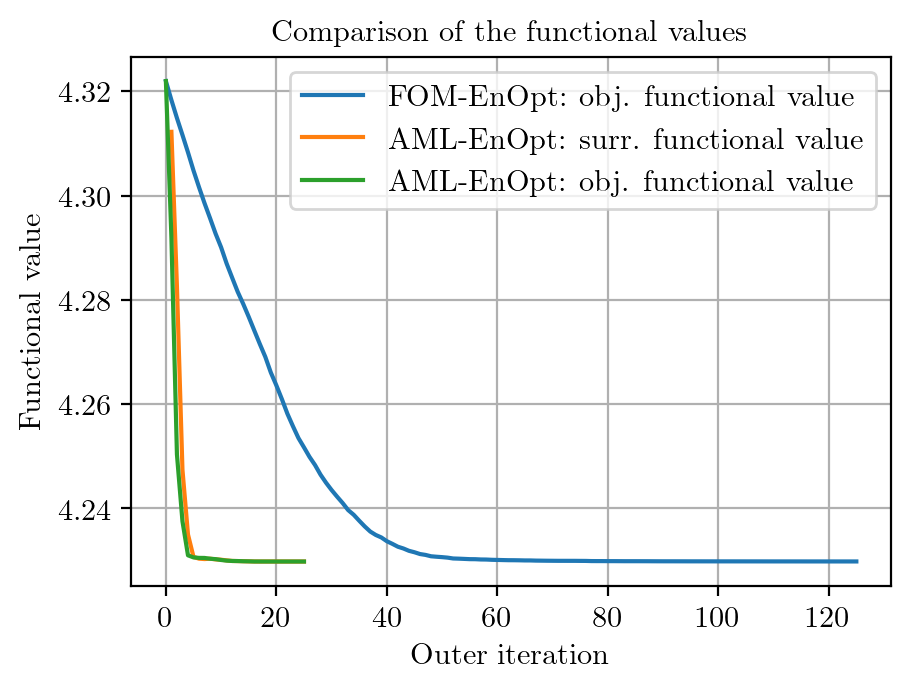
\includegraphics{Plots/functionalValueComp.png}
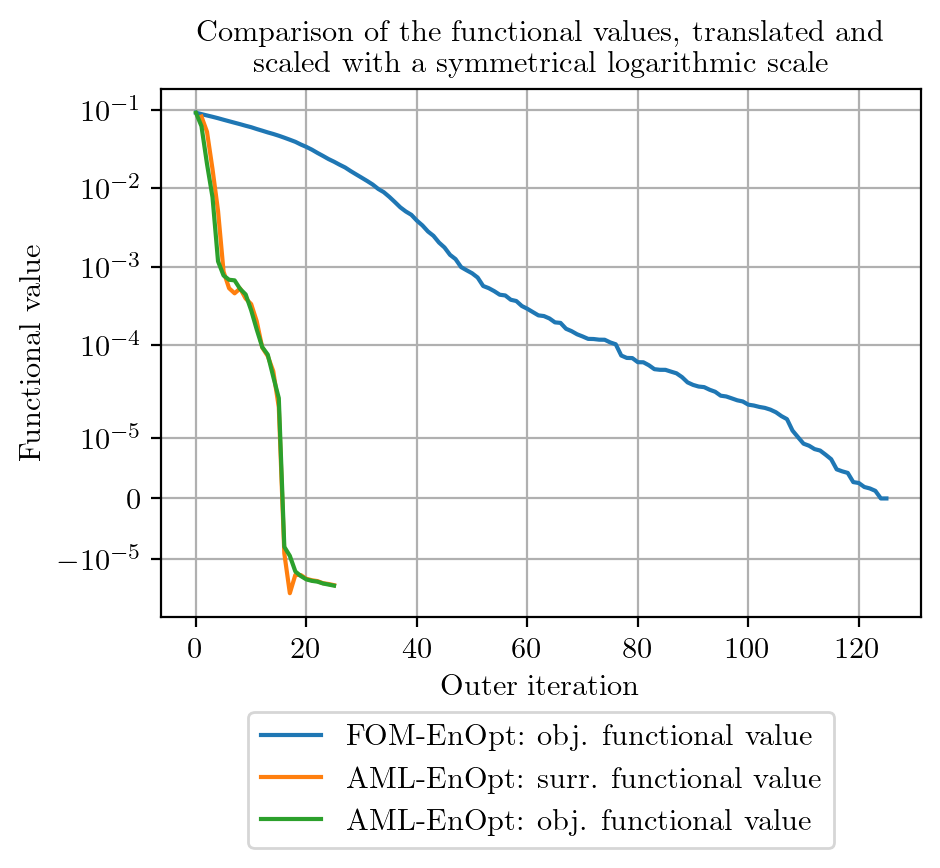
\includegraphics{Plots/functionalValueCompSymlog.png}
\caption{\label{FOMAMLEnOptFuncValComp}The FOM objective functional values obtained during the outer iterations of both EnOpt algorithms and the surrogate functional values obtained during the outer iterations of the AML-EnOpt algorithm at the top. The plot at the bottom shows these values, translated by the objective functional value of the FOM-EnOpt output and scaled with a symmetrical logarithmic scale which is linear at values which are closer to zero than the absolute value of the difference between the objective functional values of the FOM- and AML-EnOpt outputs.}
\end{figure}

We can see here that the functional values of the FOM-EnOpt and the Adaptive-ML-EnOpt algorithms converge towards a minimum. The FOM-EnOpt algorithm gives an output whose objective functional value is approximately $4.22982802$ after $125$ iterations. The FOM objective functional value of the output from the AML-EnOpt procedure is approximately $4.22981359$ which is reached after only $25$ outer iterations. So the Adaptive-EnOpt algorithm gives here not only an output that has a smaller objective functional value, but also requires far fewer outer iterations than the FOM-EnOpt algorithm to terminate.\\

To compare the functional values of the objective functional and the surrogate functionals of the Adaptive-ML-EnOpt procedure, we examine Figure \ref{AMLEnOptFuncValComp}. The plot at the top shows the same graphs as the first plot in Figure \ref{FOMAMLEnOptFuncValComp}, except that the objective functional values of the FOM-EnOpt algorithm are not included. The plot at the bottom shows only the last five outer iterations of the plot from above. We can see here that there is quite a large difference between the objective functional values and the surrogate functional values in the first outer iterations. The difference after the first iteration is approximately $0.02$. However, this difference gets smaller during the runtime of the procedure and is in the order of $10^{-7}$ during the last iterations. One exception is the iteration $17$, where the FOM objective functional value is approximately $4.22981852$ and the surrogate functional value about $4.22981001$. The difference between these values is here relatively large compared to the iterations nearby. This can be seen in Figure \ref{AMLEnOptFuncValCompSymlog} which shows the values of the plot at the top of Figure \ref{AMLEnOptFuncValComp} with a symmetrical logarithmic scale.

\begin{figure}
\centering
%\textbf{Your title}\par\medskip
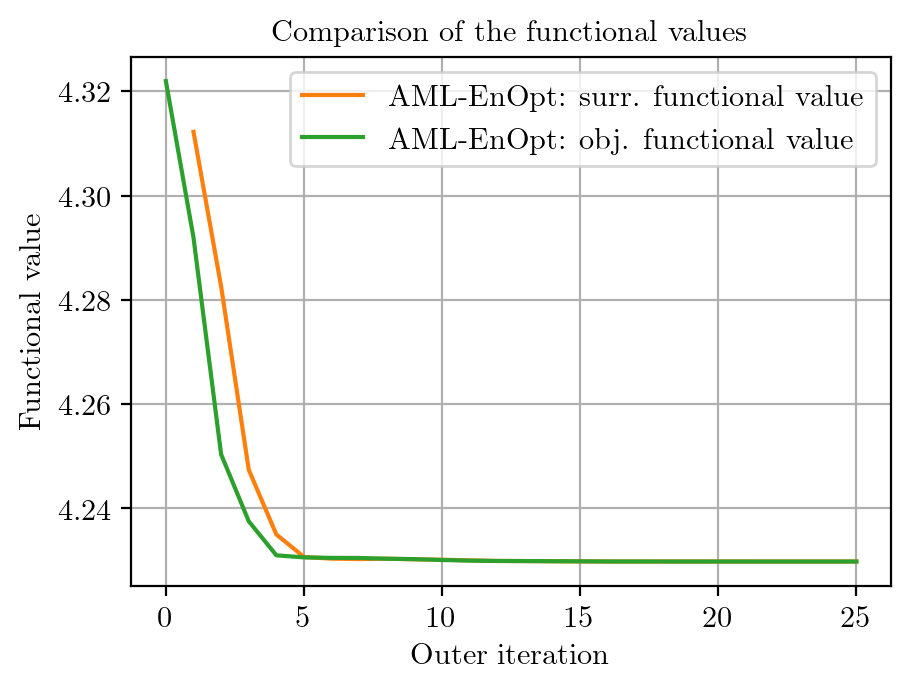
\includegraphics{Plots/reducedFunctionalValueComp.png}
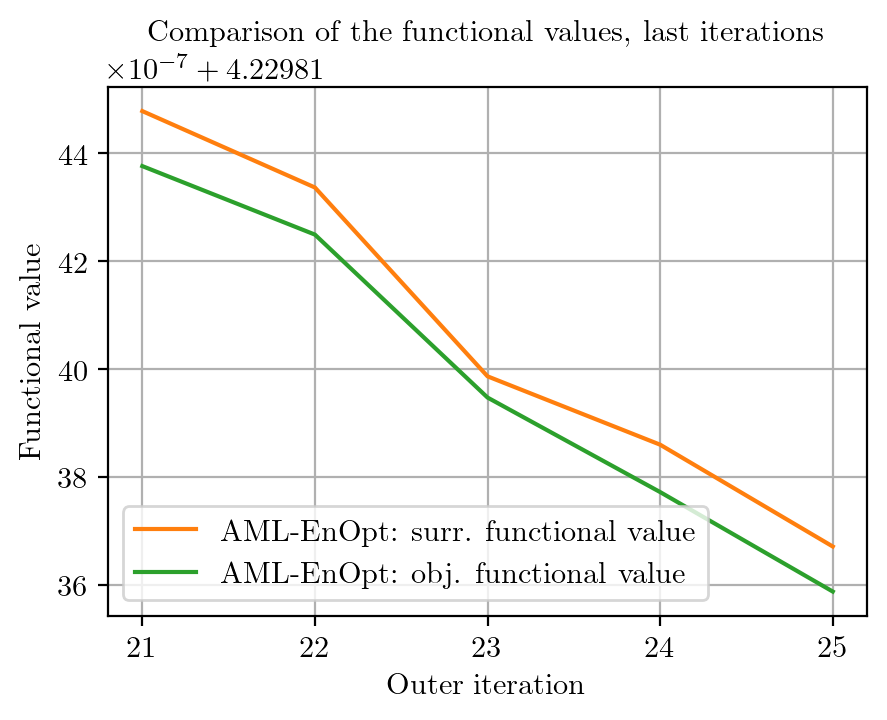
\includegraphics{Plots/reducedFunctionalValueCompLastIter.png}
\caption{\label{AMLEnOptFuncValComp}Comparison of the FOM objective functional values obtained during the outer iterations of the AML-EnOpt algorithm, as well as the respective surrogate functional values}
\end{figure}

\begin{figure}
\centering
%\textbf{Your title}\par\medskip
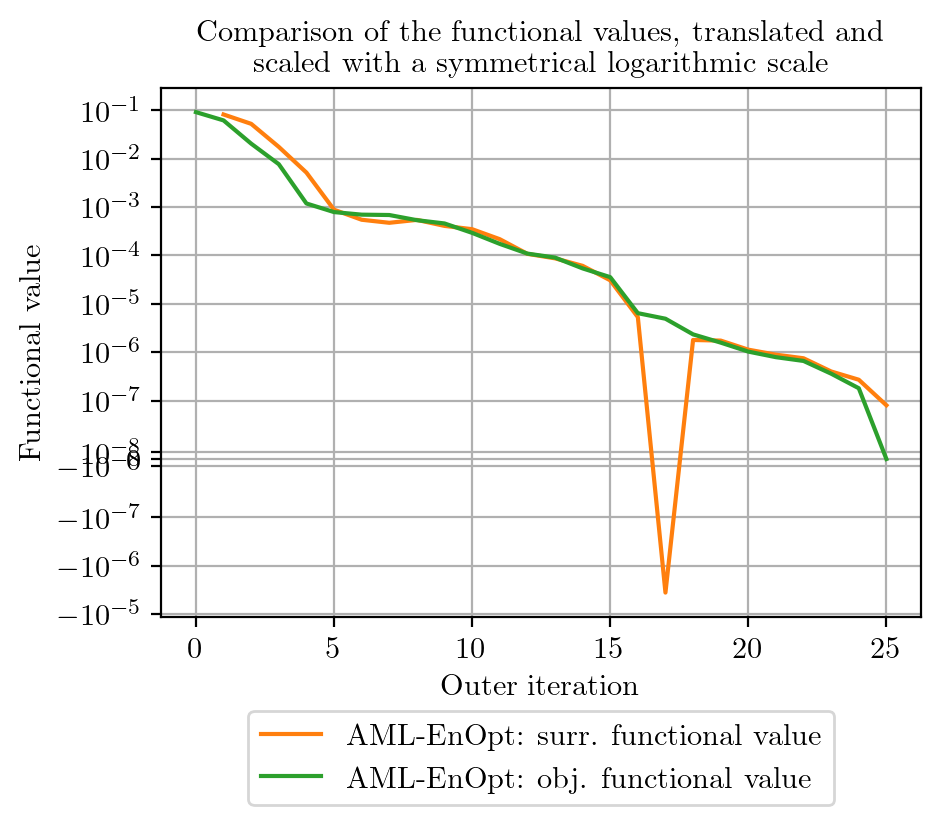
\includegraphics{Plots/reducedFunctionalValueCompSymlog.png}
\caption{\label{AMLEnOptFuncValCompSymlog}Comparison of the FOM objective functional values obtained during the outer iterations of the AML-EnOpt algorithm, as well as the respective surrogate functional values, translated by the objective functional value of the AML-EnOpt output and scaled with a symmetrical logarithmic scale which is linear at values that are closer to zero than the absolute value of the difference between the objective and surrogate functional values of the AML-EnOpt output.}
\end{figure}

One reason for the improving accuracy of the surrogate functional at the iterates is the difference between $\mathbf{q}_k$ and $\mathbf{q}^\mathrm{next}_k$ at different outer iterations. In the first iterations, we are relatively far from an optimum and therefore the iterates change considerably. The surrogate functional is trained by a training and a validation set which are sampled around the iterate $\mathbf{q}_k$, so  if the difference between $\mathbf{q}^\mathrm{next}_k$ and $\mathbf{q}_k$ is large, the same tends to hold for the difference between $\mathbf{q}^\mathrm{next}_k$ and the samples, so the surrogate functional is less precise at $\mathbf{q}^\mathrm{next}_k$. As the algorithm progresses, the iterates converge towards an optimum and the differences between successive iterates are smaller, resulting in more accurate surrogate functional values.

This can be seen in Figure \ref{L2Dist}. In the first iteration, the step from $\mathbf{q}_k$ to $\mathbf{q}^\mathrm{next}_k$ is much larger than the step from $\mathbf{q}_k$ to $\tilde{\mathbf{q}}_k$ with respect to the $L^2$-norm. The same holds with regard to the difference between $\mathbf{q}_k$ and the samples in $T_k$. Therefore the DNN is inaccurate at $\mathbf{q}^\mathrm{next}_k$. If this were the FOM-EnOpt algorithm, then $\tilde{\mathbf{q}}_k$ would be the next iterate, so we can see here a reason why the AML-EnOpt algorithm requires far fewer iterations than the FOM-EnOpt procedure which is that the machine learning-based algorithm takes larger steps at the beginning.

Although the step from $\mathbf{q}_k$ to $\mathbf{q}^\mathrm{next}_k$ is still larger than the step from $\mathbf{q}_k$ to $\tilde{\mathbf{q}}_k$ at the last iteration, the step sizes differ not by a lot compared to the first iteration. $\mathbf{q}^\mathrm{next}_k$ is even closer to $\mathbf{q}_k$ than all the samples are since the value of $\mathbf{q}^\mathrm{next}_k$ at the bottom plot in Figure \ref{L2Dist} is smaller than the value of $T_k$ min which is the sample in $T_k$ with the minimum $L^2$-distance to $\mathbf{q}_k$.\\

\begin{figure}
\centering
%\textbf{Your title}\par\medskip
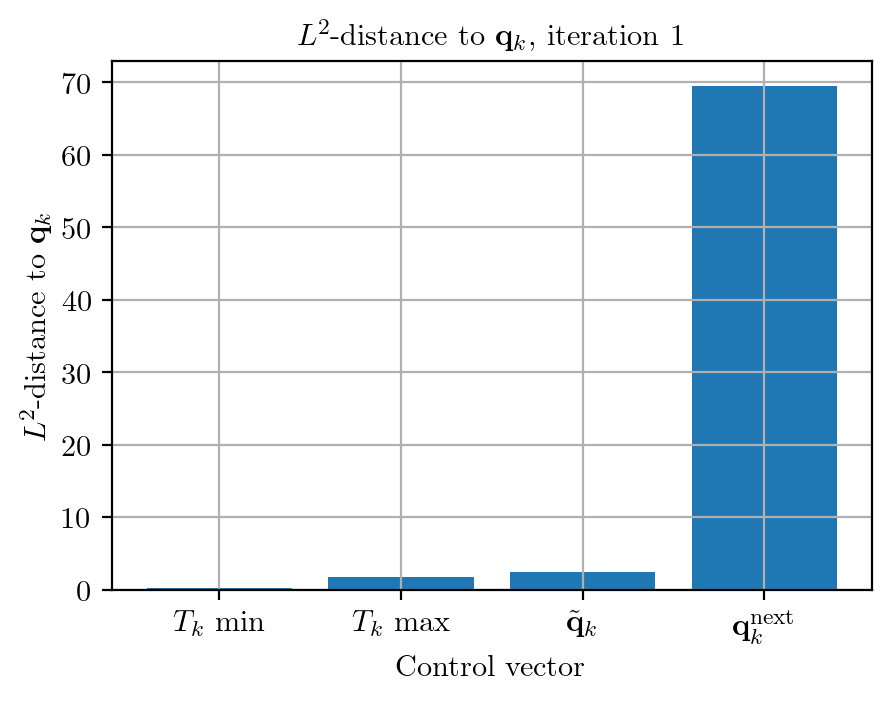
\includegraphics{Plots/firstL2Dist.png}
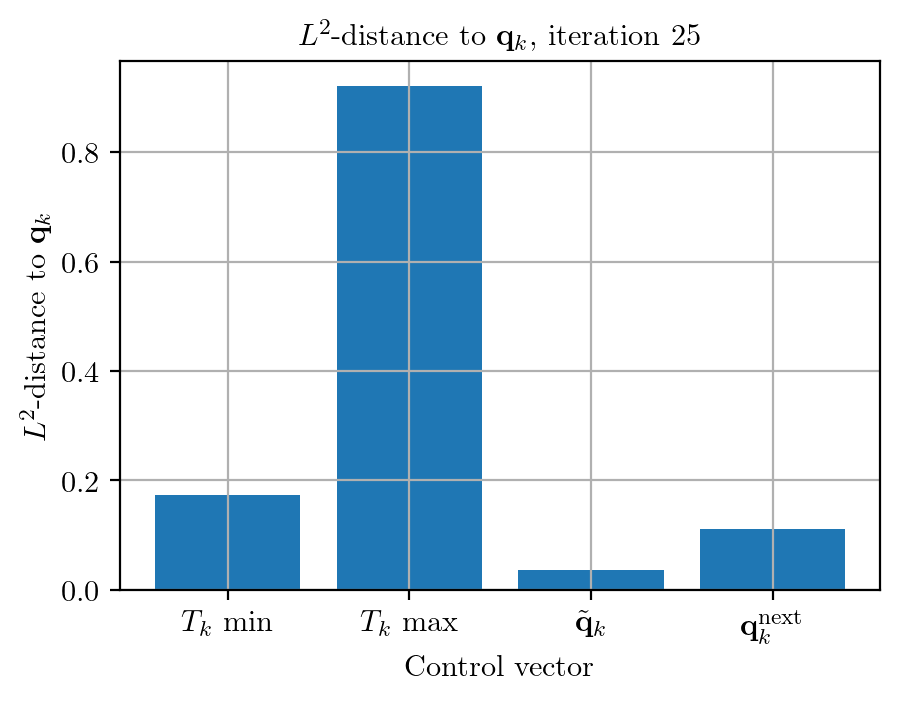
\includegraphics{Plots/lastL2Dist.png}
\caption{\label{L2Dist}$L^2$-distance between $\mathbf{q}_k$ and $T_k$ min, $T_k$ max, $\tilde{\mathbf{q}}_k$ and $\mathbf{q}^\mathrm{next}_k$ at the first (top) and last (bottom) outer iteration. $\mathbf{q}_k$ is here the iterate at the start of the respective iteration and $\mathbf{q}^\mathrm{next}_k$ the iterate at the end of the iteration. $T_k$ min is the sample in $T_k$ with the minimum $L^2$-distance to $\mathbf{q}_k$ and $T_k$ max the sample with the maximum $L^2$-distance to $\mathbf{q}_k$.}
\end{figure}

The analytical solution is not necessarily the optimal solution. To get an optimal solution as a reference, we use the L-BFGS-B minimizer \cite{doi:10.1137/0916069, 10.1145/279232.279236, 10.1145/2049662.2049669} from the Python package SciPy. The stopping criterion is here chosen so that this algorithm terminates when the maximum norm of the gradient is smaller than $10^{-7}$. This gives us an objective functional value of approximately $4.22981275$ which is reached after a runtime of only $1.28$ minutes. Both the objective functional value and the runtime of the L-BFGS-B optimizer are smaller than the values that we get from the FOM- and AML-EnOpt algorithms. Therefore, we conclude that the L-BFGS-B aglorithm is a better optimization method for this optimization problem than the EnOpt algorithms.

To measure the performance of the FOM- and AML-EnOpt algorithms, we run these procedures three times each. The results are presented in Table \ref{resultComparison}. Entries in the columns `obj. func. absolute error $(\cdot 10^{-7})$' and `obj. func. relative error $(\cdot 10^{-7})$' state the scaled absolute, respectively relative, error between the objective functional value of the respective EnOpt solution and the objective functional value of the L-BFGS-B solution that we specified above by $4.22981275$. These entries have to be multiplied by $10^{-7}$ to obtain the correct errors. In this table, the objective functional values of the AML-EnOpt procedures are all smaller and much closer to the L-BFGS-B objective functional value than the results of the FOM-EnOpt algorithm. Since the numbers of outer iterations of the AML-EnOpt procedures are significantly lower than those of the FOM-EnOpt procedures, their respective numbers of FOM evaluations are also considerably smaller. This leads to a decrease of the total run times compared to the FOM-EnOpt procedures. In our results, the training time of the AML-EnOpt procedures is more than half as long as their total run time.\\

\begin{table}
\caption{\label{resultComparison}Comparison of the results from the FOM-EnOpt and AML-EnOpt algorithms}
%\footnotesize
\centering
\begin{tabular}{|l|l|l|l|}
\hline
Method & Result & FOM objective functional value  & Surrogate functional value \\%& FOM eval. & Surrogate eval. & Training time (min) & $T_\mathrm{total}$ (min) & Speedup\\
\hline
\hline
$\mathrm{FOM-EnOpt}$ & $1$ & $4.22982619$ & - \\%& $2839$ & - & - & $54.86$ & - \\
\cline{2-4}
 & $2$ & $4.22982927$ & - \\%& $2839$ & - & - & $54.86$ & - \\
\cline{2-4}
 & $3$ & $4.22983618$ & - \\%& $2839$ & - & - & $54.86$ & - \\
 \hline
$\mathrm{AML-EnOpt}$ & $1$ & $4.2298133$ & $4.22981349$ \\%& $407$ & $12315$ & $2.03$ & $8.87$ & $6.18$ \\
\cline{2-4}
 & $2$ & $4.2298136$ & $4.22981371$ \\%& $2839$ & - & - & $54.86$ & - \\
\cline{2-4}
 & $3$ & $4.22981313$ & $4.22981329$ \\%& $2839$ & - & - & $54.86$ & - \\
\hline
\multicolumn{4}{l}{}\\
\hline
Method & Result & obj. func. absolute error $(\cdot 10^{-7})$ & obj. func. relative error $(\cdot 10^{-7})$\\%& FOM eval. & Surrogate eval. & Training time (min) & $T_\mathrm{total}$ (min) & Speedup\\
\hline
\hline
$\mathrm{FOM-EnOpt}$ & $1$ & $134.45$ & $31.79$  \\%& $2839$ & - & - & $54.86$ & - \\
\cline{2-4}
 & $2$ & $165.20$ & $39.06$ \\%& $2839$ & - & - & $54.86$ & - \\
\cline{2-4}
 & $3$ & $234.32$ & $55.40$ \\%& $2839$ & - & - & $54.86$ & - \\
 \hline
$\mathrm{AML-EnOpt}$ & $1$ & $5.48$ & $1.30$ \\%& $407$ & $12315$ & $2.03$ & $8.87$ & $6.18$ \\
\cline{2-4}
 & $2$ & $8.47$ & $2.00$ \\%& $2839$ & - & - & $54.86$ & - \\
\cline{2-4}
 & $3$ & $3.77$ & $0.89$ \\%& $2839$ & - & - & $54.86$ & - \\
\hline
\multicolumn{4}{l}{}\\
\hline
Method & Result & Outer iterations  & Inner iterations \\%& FOM eval. & Surrogate eval. & Training time (min) & $T_\mathrm{total}$ (min) & Speedup\\
\hline
\hline
$\mathrm{FOM-EnOpt}$ & $1$ & $119$ & - \\%& $2839$ & - & - & $54.86$ & - \\
\cline{2-4}
 & $2$ & $114$ & - \\%& $2839$ & - & - & $54.86$ & - \\
\cline{2-4}
 & $3$ & $124$ & - \\%& $2839$ & - & - & $54.86$ & - \\
 \hline
$\mathrm{AML-EnOpt}$ & $1$ & $27$ & $924$ \\%& $407$ & $12315$ & $2.03$ & $8.87$ & $6.18$ \\
\cline{2-4}
 & $2$ & $27$ & $877$ \\%& $2839$ & - & - & $54.86$ & - \\
\cline{2-4}
 & $3$ & $24$ & $895$ \\%& $2839$ & - & - & $54.86$ & - \\
\hline
\multicolumn{4}{l}{}\\
\hline
Method & Result & FOM evaluations  & Surrogate evaluations \\%& FOM eval. & Surrogate eval. & Training time (min) & $T_\mathrm{total}$ (min) & Speedup\\
\hline
\hline
$\mathrm{FOM-EnOpt}$ & $1$ & $12107$ & - \\%& $2839$ & - & - & $54.86$ & - \\
\cline{2-4}
 & $2$ & $11629$ & - \\%& $2839$ & - & - & $54.86$ & - \\
\cline{2-4}
 & $3$ & $12643$ & - \\%& $2839$ & - & - & $54.86$ & - \\
 \hline
$\mathrm{AML-EnOpt}$ & $1$ & $2912$ & $95047$ \\%& $407$ & $12315$ & $2.03$ & $8.87$ & $6.18$ \\
\cline{2-4}
 & $2$ & $2905$ & $90241$ \\%& $2839$ & - & - & $54.86$ & - \\
\cline{2-4}
 & $3$ & $2589$ & $91967$ \\%& $2839$ & - & - & $54.86$ & - \\
\hline
\multicolumn{4}{l}{}\\
\hline
Method & Result & Total run time (min) & Training time (min)\\%& FOM eval. & Surrogate eval. & Training time (min) & $T_\mathrm{total}$ (min) & Speedup\\
\hline
\hline
$\mathrm{FOM-EnOpt}$ & $1$ & $37.67$ & -  \\%& $2839$ & - & - & $54.86$ & - \\
\cline{2-4}
 & $2$ & $36.07$ & - \\%& $2839$ & - & - & $54.86$ & - \\
\cline{2-4}
 & $3$ & $39.22$ & - \\%& $2839$ & - & - & $54.86$ & - \\
 \hline
$\mathrm{AML-EnOpt}$ & $1$ & $24.05$ & $14.24$ \\%& $407$ & $12315$ & $2.03$ & $8.87$ & $6.18$ \\
\cline{2-4}
 & $2$ & $23.87$ & $14.17$ \\%& $2839$ & - & - & $54.86$ & - \\
\cline{2-4}
 & $3$ & $22.14$ & $13.39$ \\%& $2839$ & - & - & $54.86$ & - \\
\hline
\end{tabular}
\end{table}

Figure \ref{FOMAMLEnOptSolutionComp} shows the solutions that we get from the FOM-EnOpt and the Adaptive-ML-EnOpt algorithms, as well as the analytical solution, the L-BFGS-B solution and the initialization of the iterates at the top. At the bottom, the difference between the FOM-EnOpt, respectively AML-EnOpt, solution and the analytical solution is depicted. The plot at the bottom shows us that the two solution strategies yield similar results. At most points, the solutions of both algorithms are relatively close to the analytical solution. However, the control values for the second, last and especially first time step are far away from the analytically optimal values. The optimal control vector that is returned by the L-BFGS-B algorithm and its difference with the analytical solution is shown in Figure \ref{LBFGSBSolutionComp}. This solution has similar traits as the EnOpt solutions.

\begin{figure}
\centering
%\textbf{Your title}\par\medskip
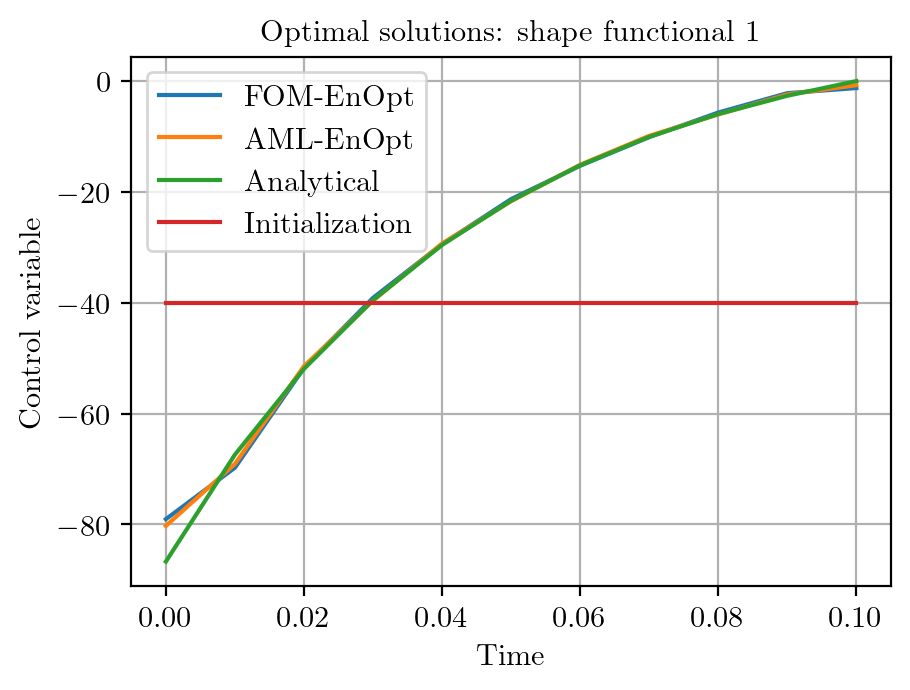
\includegraphics{Plots/solutions.png}
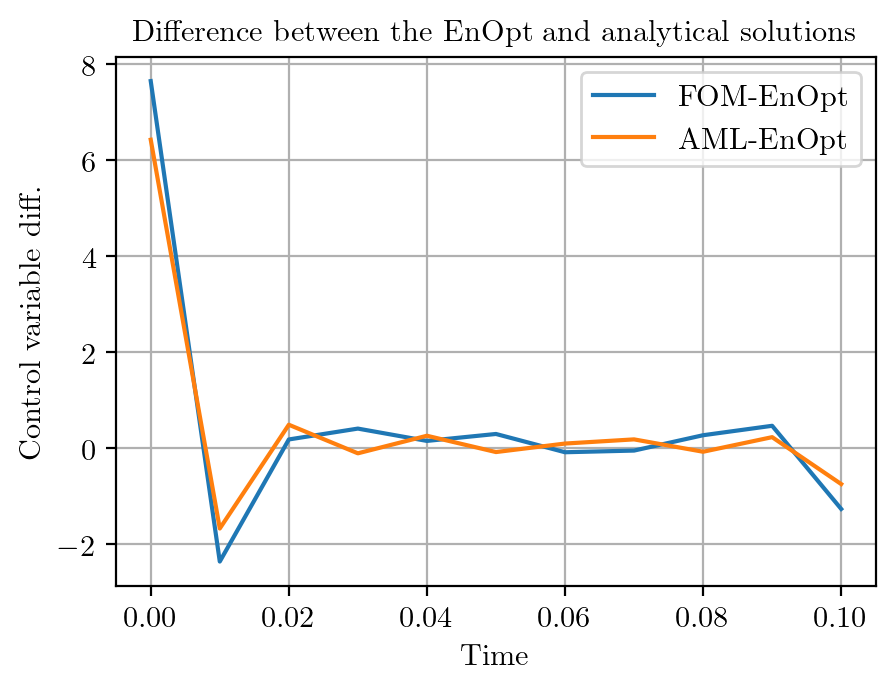
\includegraphics{Plots/solutionsDiffer.png}
\caption{\label{FOMAMLEnOptSolutionComp}Comparison of the initial value of the iterate and the optimal solutions obtained from the FOM-EnOpt, AML-EnOpt and L-BFGS-B algorithms (top) and the differences between the EnOpt solutions and the analytical solution (bottom)}
\end{figure}

\begin{figure}
\centering
%\textbf{Your title}\par\medskip
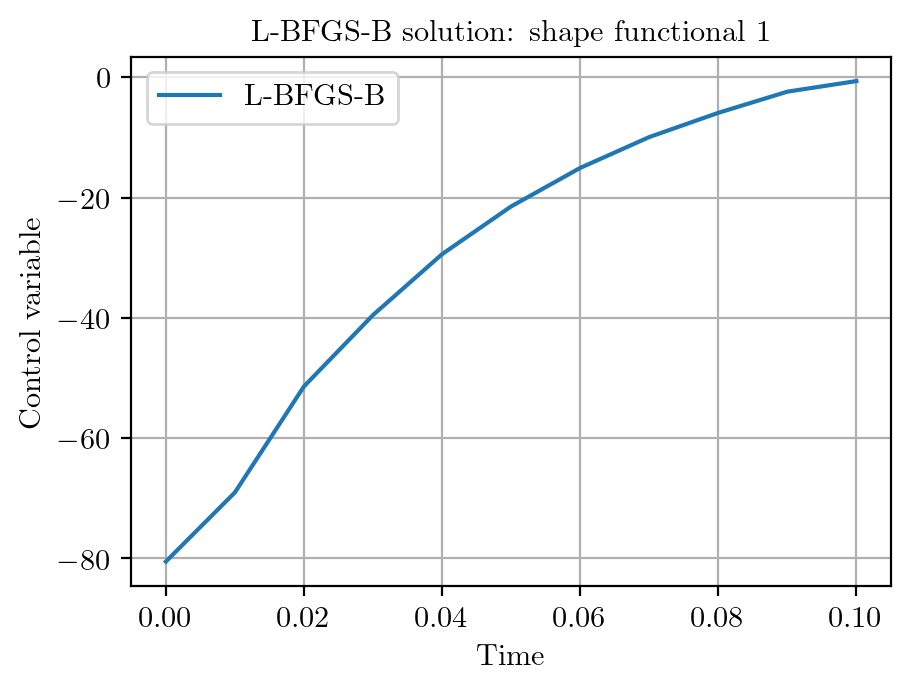
\includegraphics{Plots/LBFGSBControlVector.png}
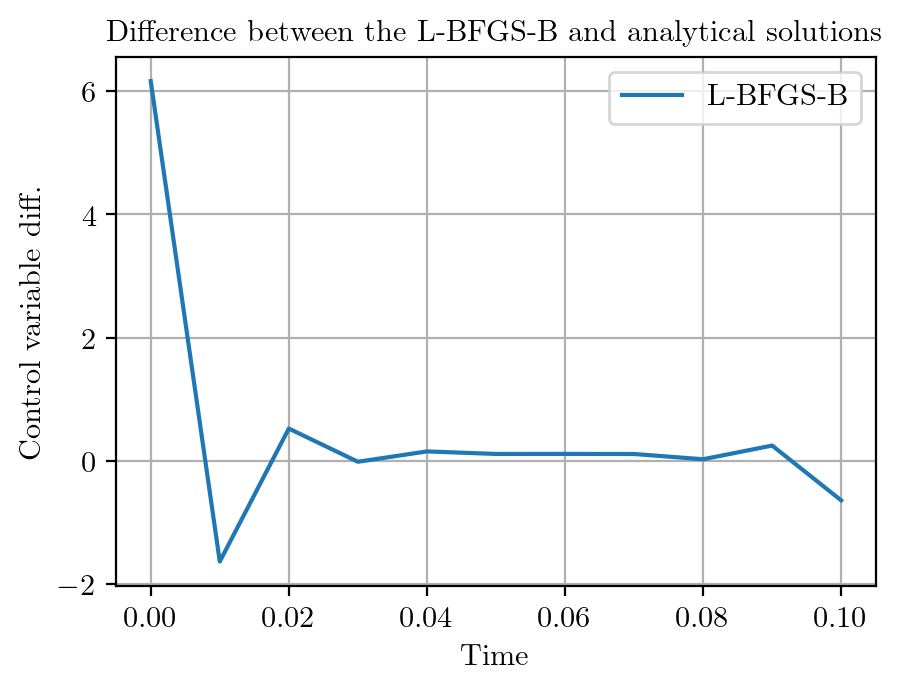
\includegraphics{Plots/LBFGSBDiffer.png}
\caption{\label{LBFGSBSolutionComp}The optimal solution obtained from the L-BFGS-B algorithm (top) and its difference with the analytical solution (bottom)}
\end{figure}

A reason for the large difference between the solutions from the optimization algorithms and the analytical solution might be inaccuracies of the state variable discretizations. The objective functional is calculated according to subsection \ref{subsectionCalculationOfTheObjectiveFunctionValue} as

\begin{equation}
\label{discretizedObjectiveFunctionalRep}
\begin{aligned}
\frac{T}{6N_t}\sum_{m=1}^{N_t}&\left(\mathbf{U}_{m-1}-\hat{\mathbf{U}}_{m-1}\right)\mathbf{M}_n\left(\mathbf{U}_{m-1}-\hat{\mathbf{U}}_{m-1}\right)\\
&+ \left(\mathbf{U}_{m-1}-\hat{\mathbf{U}}_{m-1}\right)\mathbf{M}_n\left(\mathbf{U}_{m}-\hat{\mathbf{U}}_{m}\right)\\
&+ \left(\mathbf{U}_{m}-\hat{\mathbf{U}}_{m}\right)\mathbf{M}_n\left(\mathbf{U}_{m}-\hat{\mathbf{U}}_{m}\right)\\
+ \frac{\alpha T}{6N_t}\sum_{m=1}^{N_t}&\mathbf{Q}_{m-1}\mathbf{M}_n\mathbf{Q}_{m-1} + \mathbf{Q}_{m-1}\mathbf{M}_n\mathbf{Q}_{m} + \mathbf{Q}_{m}\mathbf{M}_n\mathbf{Q}_{m},
\end{aligned}
\end{equation}
where the notation corresponds to the notation of subsection \ref{subsectionCalculationOfTheObjectiveFunctionValue}.

We compute the state vectors $\mathbf{U}_m$ with the Crank-Nicolson scheme \eqref{crank_nicolson}:
\begin{equation*}
\left(\tilde{\mathbf{M}}_n^T + \frac{T}{2N_t} \tilde{\mathbf{L}}_n^T\right) \mathbf{U}_m = \left(\tilde{\mathbf{M}}_n^T - \frac{T}{2N_t} \tilde{\mathbf{L}}_n^T\right) \mathbf{U}_{m-1} + \frac{T}{2N_t} \mathbf{F}_{m-1} + \frac{T}{2N_t} \mathbf{F}_m,
\end{equation*}
for $m=1,\dotsc,N_t$. The control $q^m_1$ influences only the vector $\mathbf{F}_m$ directly for $m=0,\dotsc,N_t$. Hence, for $m=1,\dotsc,N_t-1$, each control $q^m_1$ is used for the definitions of the states $\mathbf{U}_m$ and $\mathbf{U}_{m+1}$. Only $q^0_1$ and $q^{N_t}_1$ set just one state which is $\mathbf{U}_1$, respectively $\mathbf{U}_{N_t}$, while they are still weighted with the same value of $\frac{T}{2N_t}$ as every other control. Therefore changes of $q^0_1$ and $q^{N_t}_1$ tend to effect the first part of \eqref{discretizedObjectiveFunctionalRep} less than the other control variables. Hence, the control variables may reduce the regularization term in \eqref{discretizedObjectiveFunctionalRep} instead by going closer to zero. This can be seen for $q^0_1$. The first control of the analytical solution is approximately $\bar{q}^0_1\approx-87$ which is far from zero. Therefore, with the discretization, it might be beneficial to reduce the regularization term by increasing $q^0_1$. Since the difference $q^0_1$ and $\bar{q}^0_1$ is so large, it is not surprising that $q^1_1$ is also not a good approximation of $\bar{q}^1_1$. In contrast to $q^0_1$, $q^{N_t}_1$ is further away from zero than its respective control of the analytical solution. However, due to the quadratic nature of the regularization term, this has not such a strong effect on the objective functional value. To reduce these inaccuracies, we could increase the number of time steps. This is examined further below.\\

So far, we have compared the EnOpt solutions with the analytical solution. However, the analytical solution is not the optimum. The objective functional value of L-BFGS-B solution is smaller than the respective functional values of the EnOpt and analytical solutions. Hence, we now compare the EnOpt results with the output of the L-BFGS-B optimizer. The difference between EnOpt results and the L-BFGS-B solution is depicted in Figure \ref{EnOptLBFGSBDifferPlot}. We can see here that the AML-EnOpt solution with an average absolute error of approximately $0.09$ is closer to the L-BFGS-B solution than the FOM-EnOpt result is which has an average absolute error of about $0.42$. This is consistent with the fact that the objective functional value of the AML-EnOpt solution is smaller than the objective functional value of the FOM-EnOpt solution.\\

\begin{figure}
\centering
%\textbf{Your title}\par\medskip
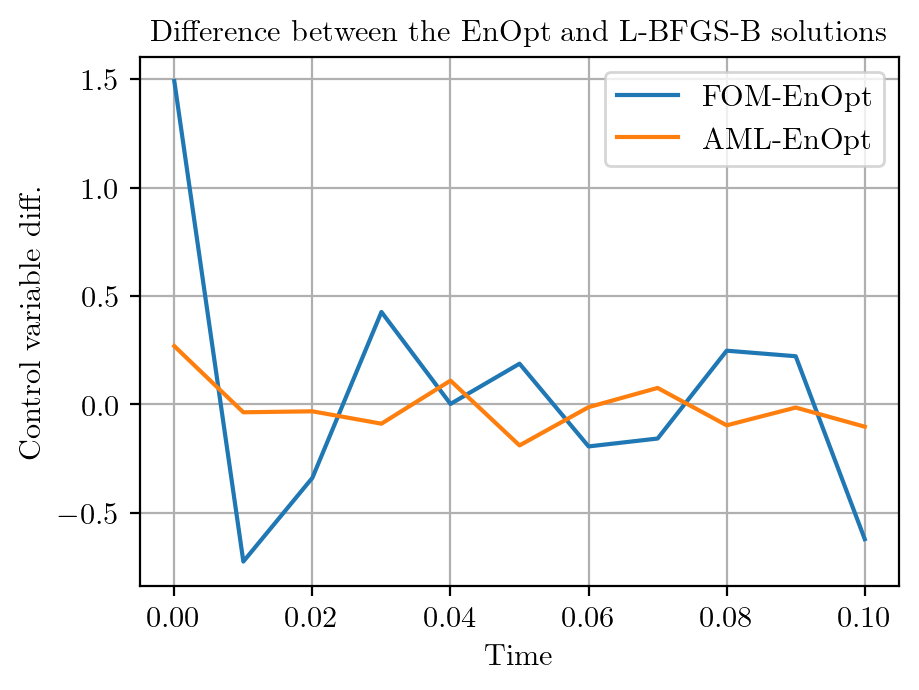
\includegraphics{Plots/EnOptLBFGSBDiffer.png}
\caption{\label{EnOptLBFGSBDifferPlot}The differences between the EnOpt solutions and the solution obtained from the L-BFGS-B optimizer}
\end{figure}

%\begin{figure}
%\centering
%%\textbf{Your title}\par\medskip
%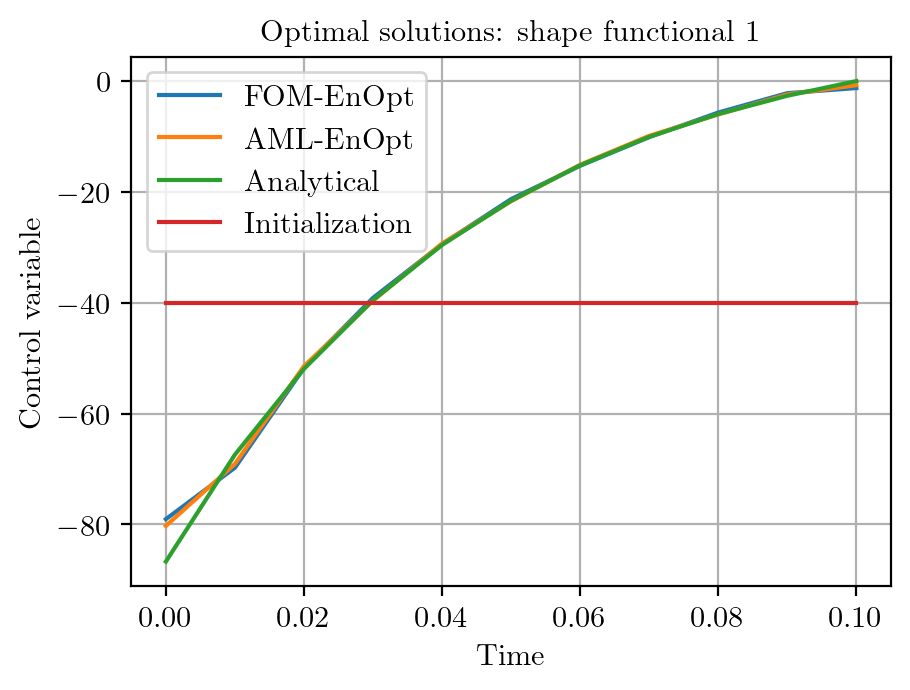
\includegraphics[height=5.7cm]{Plots/solutions.png}
%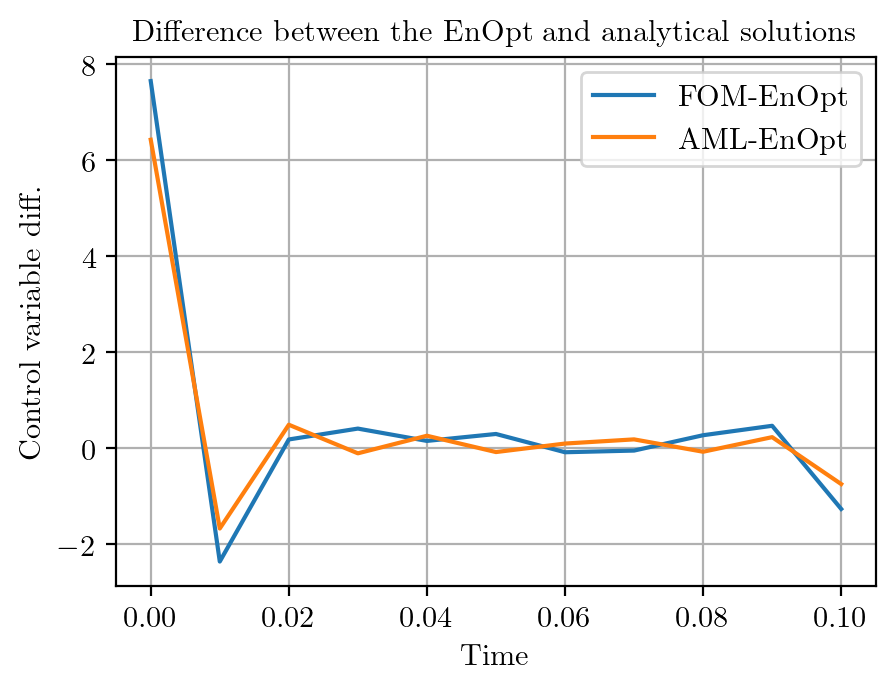
\includegraphics[height=5.7cm]{Plots/solutionsDiffer.png}
%\caption{Comparison of the optimal solutions obtained from the FOM-EnOpt and the AML-EnOpt algorithms}
%\end{figure}


To investigate the effects of different neural network structures, we test now the AML-EnOpt algorithm with different quantities of neurons in the hidden layers. The number of hidden layers is fixed to two. The progression of the FOM objective functional values for different DNN structures is shown in Figure \ref{DNNStructComparison}. To distinguish the different results, the bottom plot shows the objective functional values of the last outer iterations. Since the procedure with $1000$ neurons in the hidden layer has here many more outer iterations than the rest, we do not show this plot to make the differences between the other results clearer. The number of outer iterations, as well as the minimum, maximum, and average training and validation losses are shown in Table \ref{DNNLossComparison}. The values in the line `FOM obj. func. val. $(\cdot 10^{-5}+4.2298)$' of Table \ref{DNNStructFOMComparison}, multiplied with $10^{-5}$ and added to $4.2298$, are the FOM objective functional values that the outputs of the respective procedures yield. `Abs. err. wrt. L-BFGS-B sol.' stands for `Absolute error with respect to the L-BFGS-B solution' and `Abs. err. wrt. L-BFGS-B sol.' means `Relative error with respect to the L-BFGS-B solution' . The results that we get are not consistent but we can conclude that neual networks with a lot of neurons are not necessary to get a sufficiently good outcome. In this case, the procedures with larger neural networks have even a poorer performance than the rest. The result with $1000$ neurons in the hidden layers has by far the most outer iterations and the results with $250$ and $500$ neurons have the highest FOM objective functional values. Regarding the losses, we see that the average MSE losses on the training sets are smaller than the average losses on the validation set, but this is to be expected.\\

\begin{figure}
\centering
%\textbf{Your title}\par\medskip
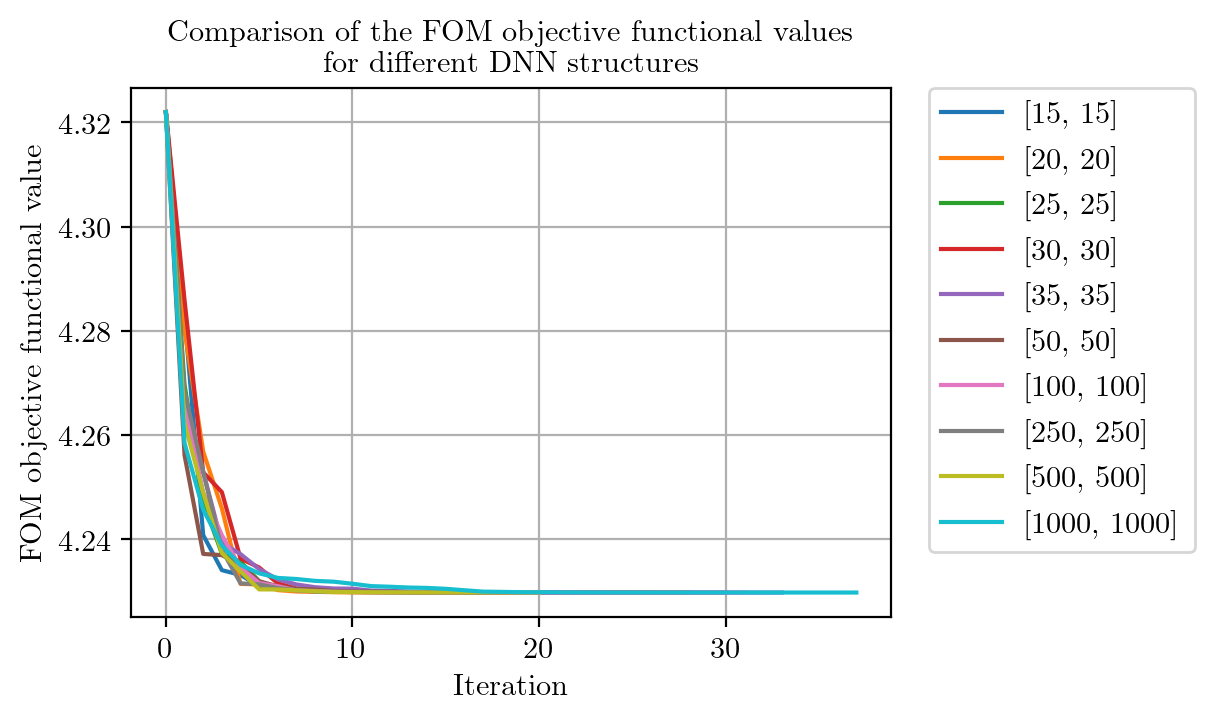
\includegraphics{Plots/DNNStruct.png}
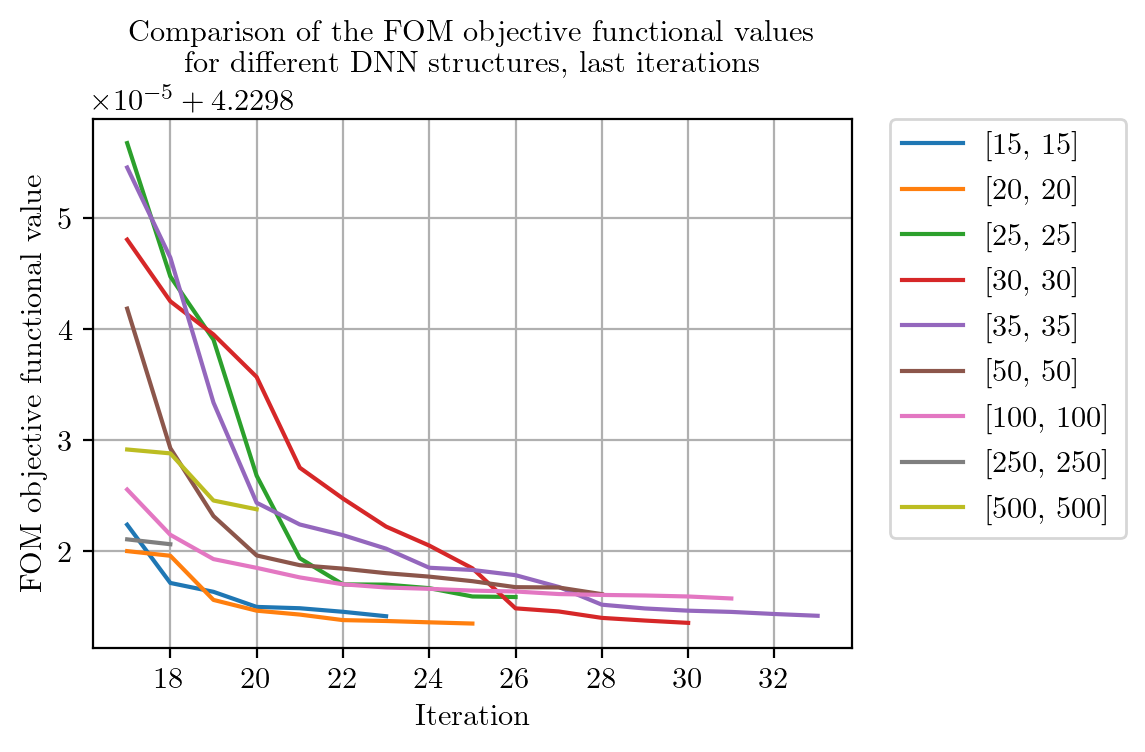
\includegraphics{Plots/DNNStructLastIter.png}
\caption{\label{DNNStructComparison}Comparison of the FOM objective functional values from the AML-EnOpt algorithm for different numbers of neurons in the hidden layers. The plot at the bottom shows the functional values of the last outer iterations without the result with $1000$ neurons in the hidden layers.}
\end{figure}


\begin{table}
\caption{\label{DNNLossComparison}Minimum, maximum, and average MSE loss on the training and validation set during the AML-EnOpt procedure with different numbers of neurons in the hidden layers of the neural network. The number of hidden layers is fixed to two.}
%\footnotesize
\centering
\begin{tabular}{|l|l|lll|lll|}
\hline
Neurons & Outer  & \multicolumn{3}{l|}{Training loss} & \multicolumn{3}{l|}{Validation loss} \\
\cline{3-5}\cline{6-8}
$N_1=N_2$ & iter. & Min. & Max. & Avg. & Min. & Max. & Avg.\\
\hline
$15$ & $23$ & $2.1\cdot10^{-7}$ & $2.6\cdot10^{-4}$ & $2.1\cdot10^{-5}$ & $7.3\cdot10^{-7}$ & $1.4\cdot10^{-3}$ & $2.5\cdot10^{-4}$\\
$20$ & $25$ & $3.3\cdot10^{-7}$ & $7.7\cdot10^{-4}$ & $6.2\cdot10^{-5}$ & $1.9\cdot10^{-6}$ & $2.9\cdot10^{-3}$ & $4.7\cdot10^{-4}$\\
$25$ & $26$ & $4.7\cdot10^{-7}$ & $9.3\cdot10^{-5}$ & $1.2\cdot10^{-5}$ & $1.0\cdot10^{-6}$ & $4.2\cdot10^{-4}$ & $1.0\cdot10^{-4}$\\
$30$ & $30$ & $3.0\cdot10^{-7}$ & $1.1\cdot10^{-4}$ & $9.4\cdot10^{-6}$ & $3.9\cdot10^{-7}$ & $1.1\cdot10^{-3}$ & $2.1\cdot10^{-4}$\\
$35$ & $33$ & $2.5\cdot10^{-7}$ & $5.7\cdot10^{-4}$ & $2.2\cdot10^{-5}$ & $9.3\cdot10^{-7}$ & $1.6\cdot10^{-3}$ & $2.0\cdot10^{-4}$\\
$50$ & $28$ & $3.9\cdot10^{-7}$ & $3.3\cdot10^{-4}$ & $2.3\cdot10^{-5}$ & $5.2\cdot10^{-7}$ & $3.6\cdot10^{-4}$ & $9.3\cdot10^{-5}$\\
$100$ & $31$ & $5.7\cdot10^{-7}$ & $6.5\cdot10^{-5}$ & $1.2\cdot10^{-5}$ & $1.3\cdot10^{-6}$ & $6.1\cdot10^{-4}$ & $1.6\cdot10^{-4}$\\
$250$ & $18$ & $2.9\cdot10^{-7}$ & $7.2\cdot10^{-5}$ & $1.1\cdot10^{-5}$ & $8.4\cdot10^{-7}$ & $5.2\cdot10^{-4}$ & $8.6\cdot10^{-5}$\\
$500$ & $20$ & $5.3\cdot10^{-7}$ & $1.3\cdot10^{-4}$ & $1.6\cdot10^{-5}$ & $6.8\cdot10^{-7}$ & $4.1\cdot10^{-4}$ & $8.9\cdot10^{-5}$\\
$1000$ & $37$ & $4.0\cdot10^{-7}$ & $9.0\cdot10^{-5}$ & $1.3\cdot10^{-5}$ & $1.4\cdot10^{-6}$ & $4.2\cdot10^{-4}$ & $9.0\cdot10^{-5}$\\
\hline
\end{tabular}
\end{table}

\begin{table}
\caption{\label{DNNStructFOMComparison} FOM objective functional output values of the AML-EnOpt procedure with different numbers of neurons in the hidden layers of the neural network. The number of hidden layers is fixed to two.}
%\footnotesize
\centering
\begin{tabular}{|l|llllllllll|}
\hline
Neurons&&&&&&&&&&\\
$(N_1=N_2)$& $15$ & $20$ & $25$ & $30$ & $35$ & $50$ & $100$ & $250$ & $500$ & $1000$\\
\hline
FOM obj.&&&&&&&&&&\\
func. val.&&&&&&&&&&\\
$(\cdot 10^{-5}+4.2298)$& $1.41$ & $1.35$ & $1.59$ & $1.35$ & $1.42$ & $1.61$ & $1.57$ & $2.06$ & $2.38$ & $1.63$\\
\hline
Abs. err. wrt.&&&&&&&&&&\\
L-BFGS-B sol.&&&&&&&&&&\\
$(\cdot 10^{-6})$& $1.38$ & $0.72$ & $3.11$ & $0.78$ & $1.42$ & $3.37$ & $2.98$ & $7.87$ & $11.02$ & $3.57$\\
\hline
Rel. err. wrt.&&&&&&&&&&\\
L-BFGS-B sol.&&&&&&&&&&\\
$(\cdot 10^{-7})$& $3.27$ & $1.70$ & $7.36$ & $1.83$ & $3.35$ & $7.96$ & $7.05$ & $18.61$ & $16.05$ & $8.44$\\
\hline
Training time&&&&&&&&&&\\
(min)& $14.01$ & $15.39$ & $15.17$ & $22.00$ & $20.99$ & $13.40$ & $17.95$ & $7.06$ & $6.59$ & $16.25$\\
\hline
Total run time&&&&&&&&&&\\
(min)& $22.44$ & $25.02$ & $25.23$ & $35.60$ & $37.66$ & $25.51$ & $35.09$ & $16.69$ & $14.51$ & $29.56$\\
\hline
\end{tabular}
\end{table}

The initial shape functional control variance $\sigma^2_1$ and the constant correlation factor $\rho$ have a strong effect on the runtime and output of the FOM-EnOpt and AML-EnOpt algorithms. If the variance is too large, the FOM-EnOpt procedure tends to give a worse optimal solution. If the variance is too small, this algorithm needs more optimization steps than necessary to terminate.

We choose the correlation factor to be close to one so that we get a smoother output. However, if this value is too large, the result is similar to a large $\sigma^2_1$ which we want to avoid. For example, if we set $\rho=0.9$, we get from \eqref{defineInitialCovariance} that the variance of $q^i_1$ is approximately $5.3\cdot\sigma^2_1$ for $i=0,\dotsc,N_t$. If $\rho$ is equal to $0.99$, the variance is with a value of approximately $50.3\cdot\sigma^2_1$ almost ten times as high.

A poor choice of these values may have even more serious consequences for the FOM-EnOpt algorithm. If we set the variance too small, the neural network-based surrogate functional is not approximating the FOM objective functional sufficiently well in a large enough area and the AML-EnOpt algorithm fails. However, we still want to set the variance so small that the surrogate is a good approximation of the objective functional in a small area around the current iterate when we are close to the optimal solution.

We conclude that $\sigma^2_1$ and $\rho$ should be chosen carefully and dependent on each other. If we increase $\rho$ to get smoother iterates, we might have to decrease $\sigma^2_1$ so that the area which contains our samples is not too large. Also, the covariance matrix adaption step size $\beta_2$ should be large enough that the samples deviate not too much when the iterates get close to the optimum but not too large since that might result in variances close to zero when the iterate is not close to the optimum. Hence, it might require some testing to find values that suit the available optimization problem.\\

Unlike the Adaptive-ML-EnOpt algorithm in \cite{Keil2022-dj}, we need to employ a trust-region method. If we proceed without it, we get the results of Figure \ref{noTRResults}. The method seems to work up to the eighth iteration, but the machine learning-based surrogate suggests in the ninth outer iteration that there is an optimum near a point that is far from the actual optimum. This point is shown in the bottom plot of Figure \ref{noTRResults}. Some entries of the resulting control vector exceed even the value of $600$, although they should be below zero.\\

\begin{figure}
\centering
%\textbf{Your title}\par\medskip
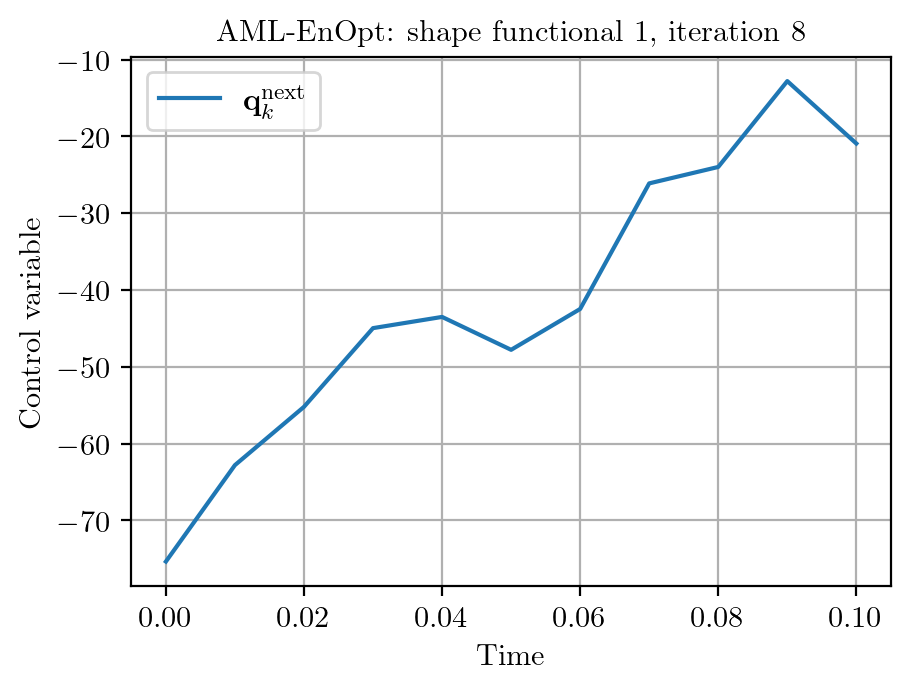
\includegraphics{Plots/noTRIteration8.png}
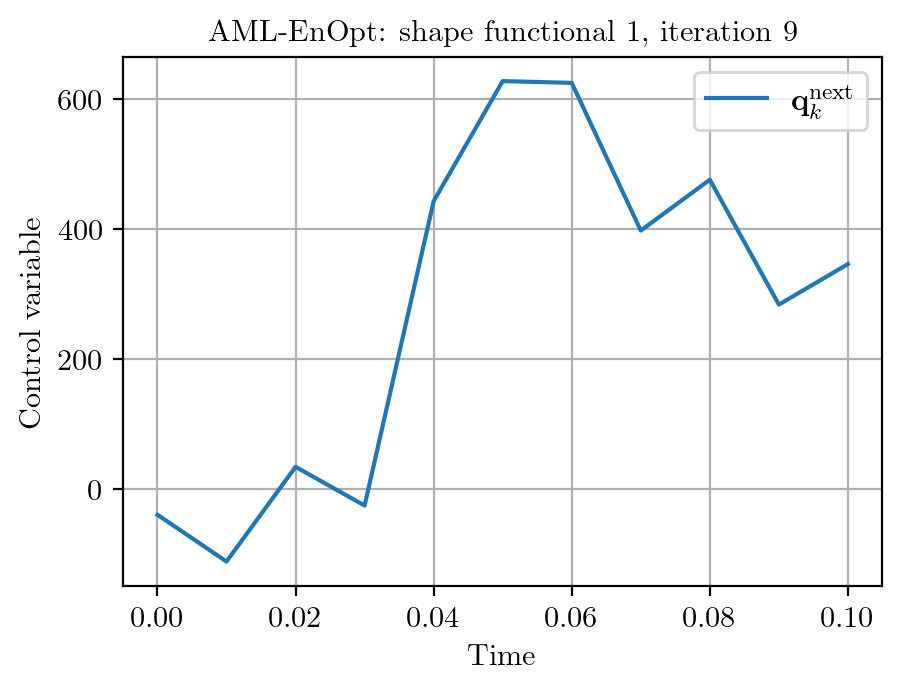
\includegraphics{Plots/noTRIteration9.png}
\caption{\label{noTRResults}An example of iterates after the eighth and ninth outer iteration of an AML-EnOpt procedure if the trust-region method is not applied}
\end{figure}

Now we compare how both algorithms get to their respective solution. During the FOM-EnOpt procedure, the iterates form a curve with a smooth shape early on. Going on, this curve changes only slightly after each iteration, mainly due to vertical stretching. With the Adaptive-ML-EnOpt method, the iterates are relatively close to the optimal point after a few iterations. Therefore, most iterations change the values of the iterates only slightly. To demonstrate this, the plots of the iterates after the fifth outer iteration are shown in Figure \ref{FOMROMEnIptIter5}. We see here that the curve of the FOM-EnOpt procedure has a much smoother shape than that of the Adaptive-ML-EnOpt method. However, the values of the FOM method iterate lie in a range between approximately $-39$ and $-35$ and are far from the optimum while their counterparts take a minimum below $-70$ and a maximum of around $0$.\\

\begin{figure}
\centering
%\textbf{Your title}\par\medskip
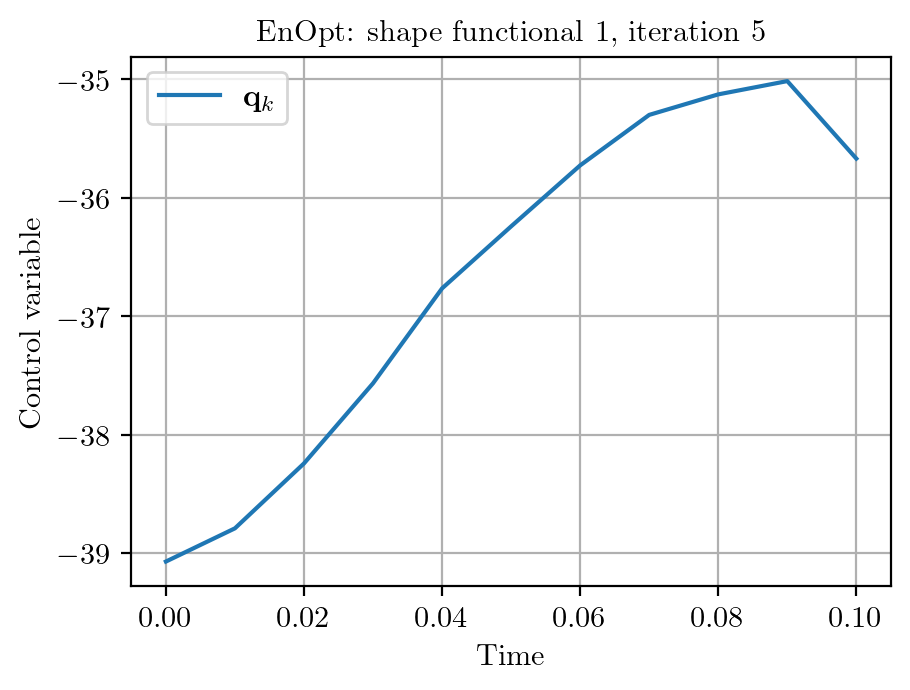
\includegraphics{Plots/FOMEnOptIter5.png}
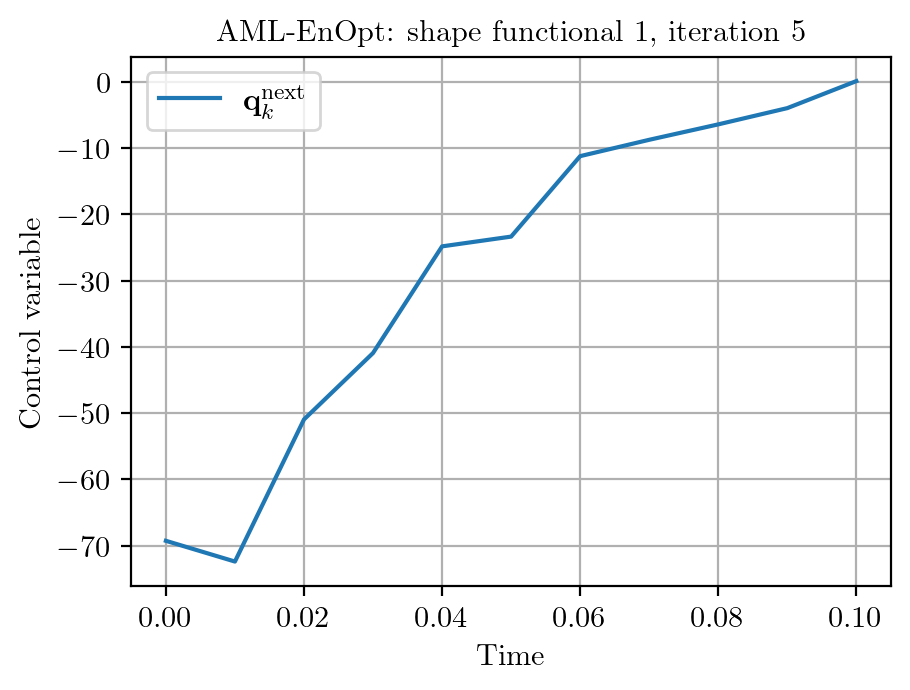
\includegraphics{Plots/ROMEnOptIter5.png}
\caption{\label{FOMROMEnIptIter5}The iterates of the FOM-EnOpt (top) and the Adaptive-ML-EnOpt (bottom) algorithms after the fifth iteration}
\end{figure}

Before we increase the number of time steps, we try out other initializations. Let $\mathbf{q}^1_0$ be the zero vector and $\mathbf{q}^2_0$ a vector where every element has the value $-90$. The solutions that we get from the FOM and the machine learning-based algorithm when we initialize the first iterate as $\mathbf{q}^1_0$ is depicted in Figure \ref{solutionsInit0}. The solution with the initialization $\mathbf{q}^2_0$ is shown in Figure \ref{solutionsInit-90}. With an initialization of $\mathbf{q}^1_0$ we get similar results for both initializations. The FOM-EnOpt procedure returns an objective functional value of approximately $4.22982378$ after $146$ outer iterations. The AML-EnOpt algorithms solution has an objective functional value of about $4.2298234$ which is reached after $24$ outer iterations. These results are similar to the outcomes of the original initialization. The biggest difference is the number of outer iterations of the FOM-EnOpt procedure. The result with the original initialization needs only $125$. The AML-EnOpt procedure with the initialization $\mathbf{q}^1_0$ terminates here even one outer iteration earlier than the first initialization, but has a larger objective functional value.

When we initialize these algorithms with $\mathbf{q}^2_0$, we get different results. The AML-EnOpt procedure still yields a similar outcome. It returns an objective functional value of approximately $4.22981306$ after $32$ outer iterations, so a few more than with the other initializations. However, the FOM-EnOpt algorithm provides a solution that is far from the optimal solution. This iterate is returned after $1000$ iterations with an objective functional value of about $4.24305956$, so the stopping criterion fulfilled in line \ref{FOMStoppingCriterionAlg} of Algorithm \ref{EnOptAlg} was $k<k^*$ instead of $F_{k}>F^\mathrm{prev}_k+\varepsilon$. We conclude from this that the quality of the AML-EnOpt output is less dependent on the initialization than that of the FOM-EnOpt algorithm.\\

\begin{figure}
\centering
%\textbf{Your title}\par\medskip
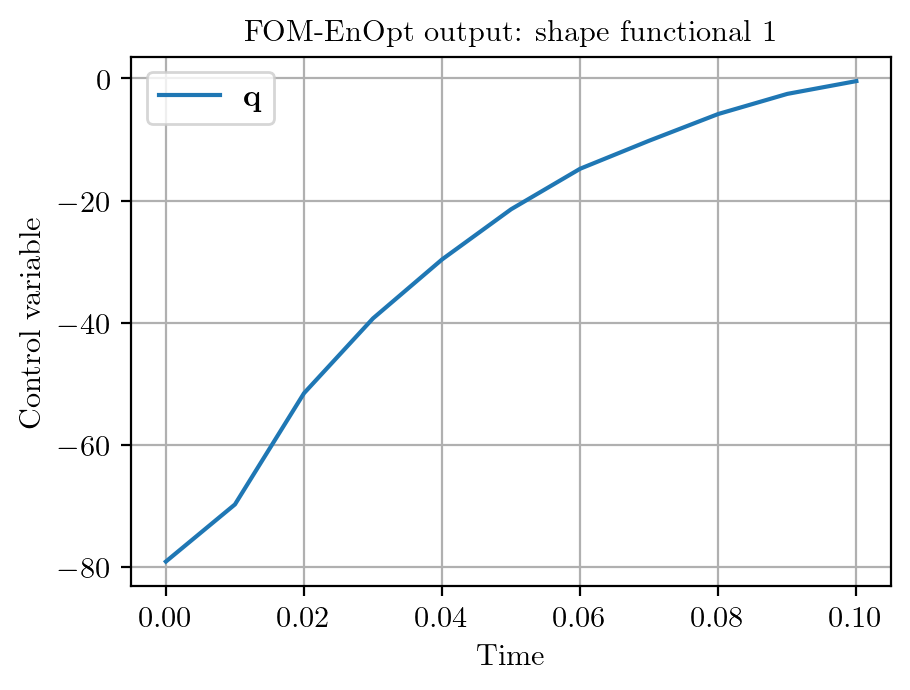
\includegraphics{Plots/FOMInit0.png}
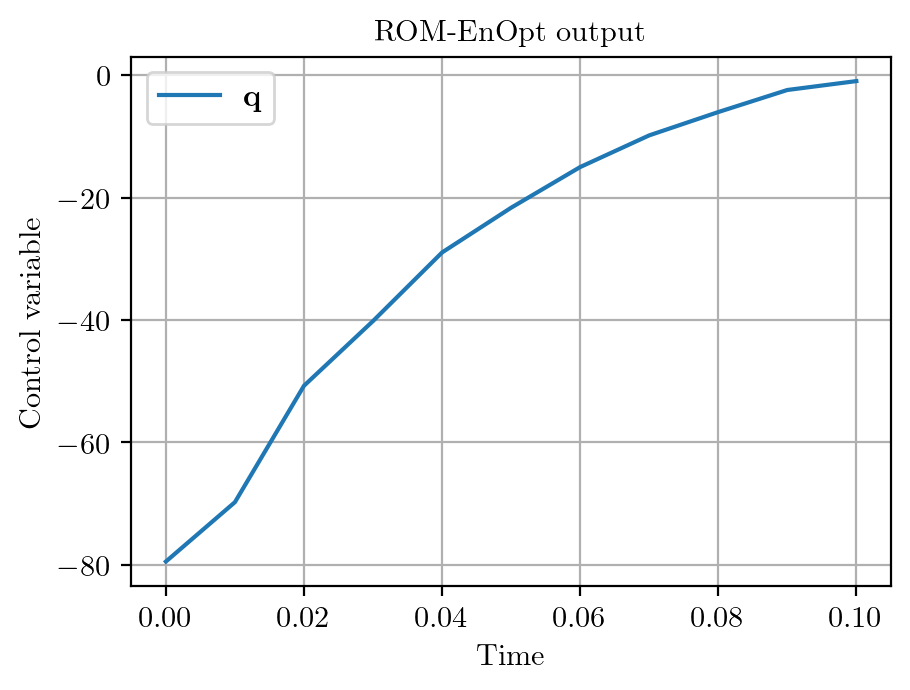
\includegraphics{Plots/ROMInit0.png}
\caption{\label{solutionsInit0}Solutions of the FOM-EnOpt (top) and AML-EnOpt (bottom) algorithms with an initialization of $\mathbf{q}^1_0$}
\end{figure}

\begin{figure}
\centering
%\textbf{Your title}\par\medskip
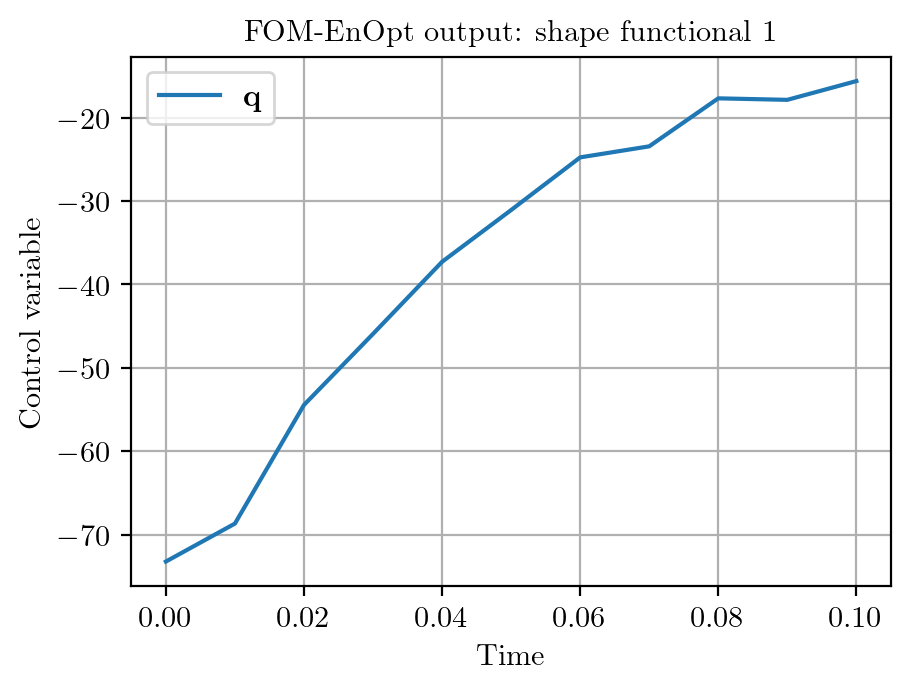
\includegraphics{Plots/FOMInit-90.png}
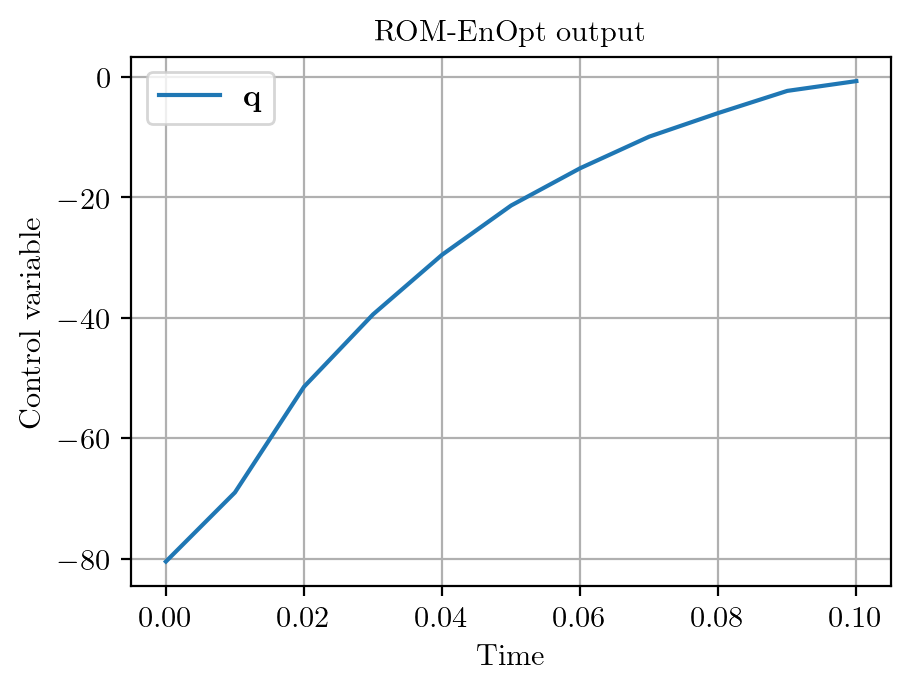
\includegraphics{Plots/ROMInit-90.png}
\caption{\label{solutionsInit-90}Solutions of the FOM-EnOpt (top) and AML-EnOpt (bottom) algorithms with an initialization of $\mathbf{q}^2_0$}
\end{figure}

Now we increase the number of time steps. That means we set $N_t=50$ which gives us control vectors of the size $N_\mathbf{q}=51$. This increases the time it takes to compute a FOM objective functional value. Therefore, we also increase the time to train a neural network for the surrogate functional by setting the number of training restarts to $10$. The other neural network training parameters are like we described it above. The non-DNN-specific parameters are set according to Table \ref{FOMAMLEnOptParametersNT50}. During the testing we had the problem that the solutions were not smooth enough. Especially the results of the AML-EnOpt algorithm were bad. Therefore we increase the correlation coefficient $\rho$ to $0.99$ and thus we must decrease the initial variance $\sigma^2_1$ to a smaller number which is here $0.01$. Also, a decrease of the covariance matrix adaption step size to $0.001$ gives us better results. Nevertheless, the FOM- and especially the AML-EnOpt solutions are still not very smooth, as it is shown in Figure \ref{solutionsNT50}, which depicts these solutions. Still, the AML-EnOpt solution yields a smaller objective functional value as it is shown below.

\begin{figure}
\centering
%\textbf{Your title}\par\medskip
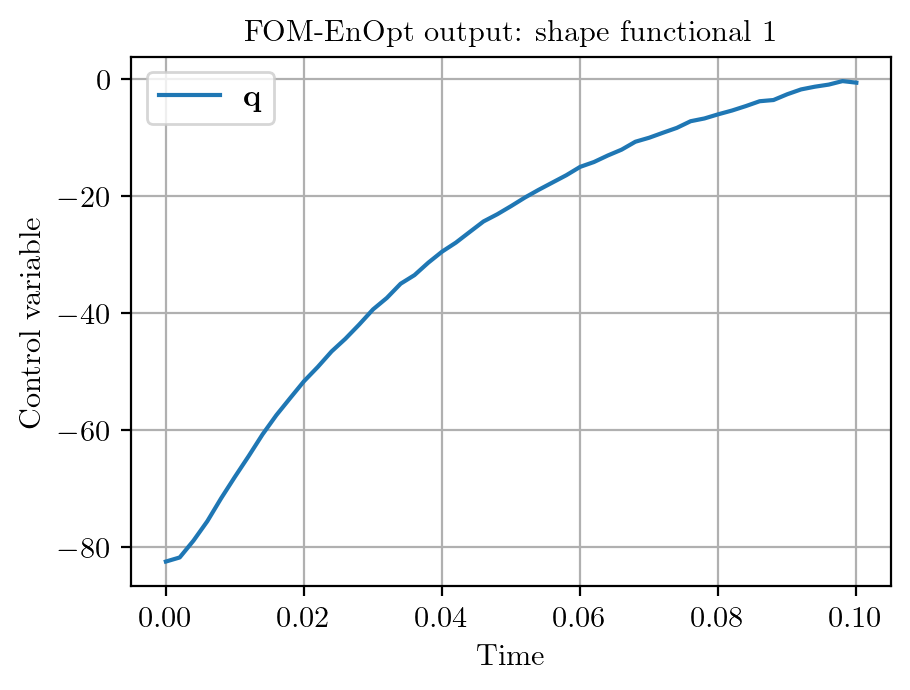
\includegraphics{Plots/FOMSolutionNT50.png}
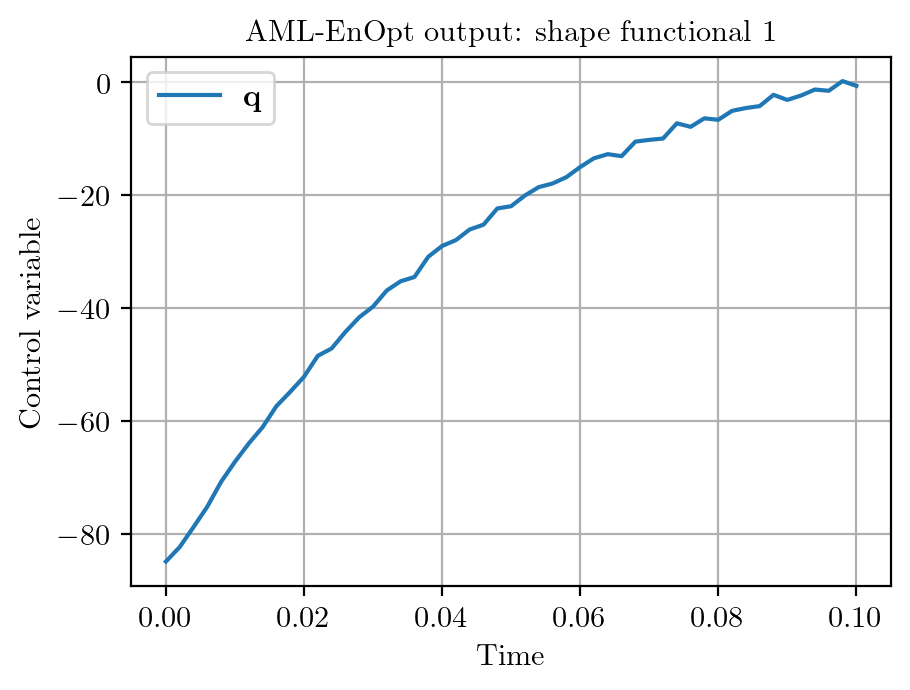
\includegraphics{Plots/ROMSolutionNT50.png}
\caption{\label{solutionsNT50}Solutions of the FOM-EnOpt (top) and AML-EnOpt (bottom) algorithms with $50$ time steps}
\end{figure}

The FOM-EnOpt procedure terminates after a runtime of $445.99$ minutes and its solution has a FOM objective functional value of approximately $4.20986746$. The objective functional value of the AML-EnOpt solution is about $4.20986518$ which is returned after a total runtime of $232.9$ minutes and a training time of $146.99$ minutes. The L-BFGS-B algorithm terminates after only $7.71$ minutes and returns a solution with an objective functional value of approximately $4.209848$. So again, the performance of the L-BFGS-B optimizer is much better than that of the FOM-EnOpt algorithms. As in Figure \ref{FOMAMLEnOptFuncValComp}, the development of the FOM objective functional values during the runtime of the FOM- and AML-EnOpt algorithms, as well as the progression of the surrogate functional values of the AML-EnOpt procedure are shown in Figure \ref{FOMAMLEnOptFuncValCompNT50}. The solutions are depicted in Figure \ref{solutionsNT50Plot} and the differences with the analytical solution in Figure \ref{solutionsDifferNT50}. The large differences at the boundaries do still exist, but now they are less noticeable because of the increased number of time steps. The L-BFGS-B optimizer gives here a result that is closer to the analytical solution than the results of the EnOpt procedures. Figure \ref{solutionsDifferLBFGSBNT50} shows the differences between the EnOpt solutions and the L-BFGS-B solution. We see here that the FOM-EnOpt solution with an average absolute difference of about $0.27$ is closer to the L-BFGS-B solution than the output of the AML-EnOpt procedure which has an average absolute difference of approximately $0.42$. The points in the first time steps are exceptions to this observation. That is probably the reason why the AML-EnOpt objective functional value is smaller than the FOM-EnOpt functional value.\\

Summarization our results, we conclude that the Adaptive-ML-EnOpt method not only decreases the computation time, but also yields smaller objective functional values compared to the FOM-EnOpt algorithm when the input dimension is low enough. However, the AML-EnOpt algorithm as implemented here has more problems to find smooth optimal solutions when the number of time steps increases. Other parameters than the ones presented in \ref{FOMAMLEnOptParametersNT50} could provide an improvement, but this requires further testing and might change for other problems. For this problem specifically, there are better optimizers than the two EnOpt algorithms, for example the L-BFGS-B method.

\begin{figure}
\centering
%\textbf{Your title}\par\medskip
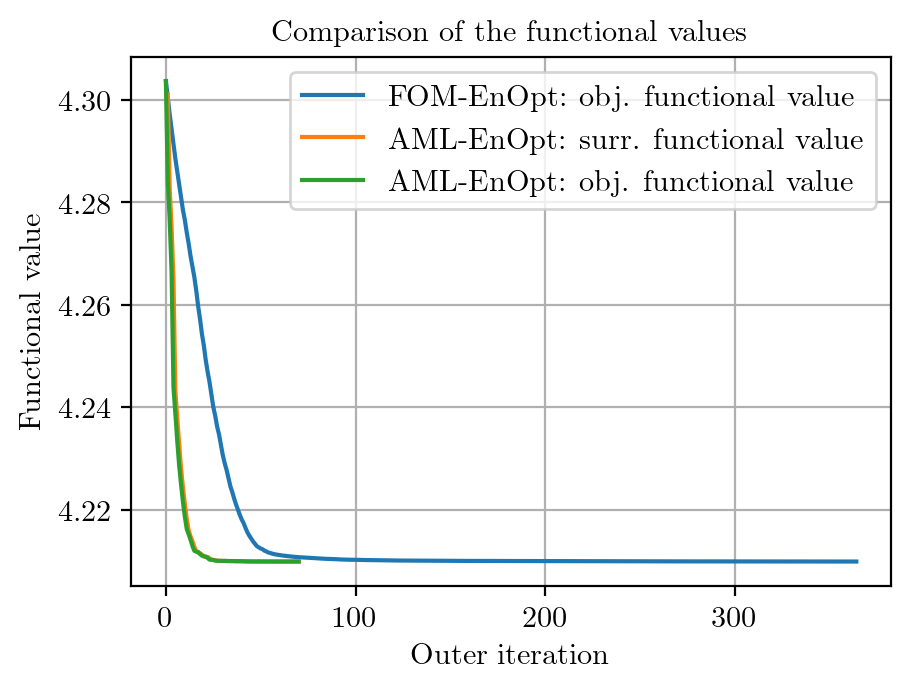
\includegraphics{Plots/functionalValueCompNT50.png}
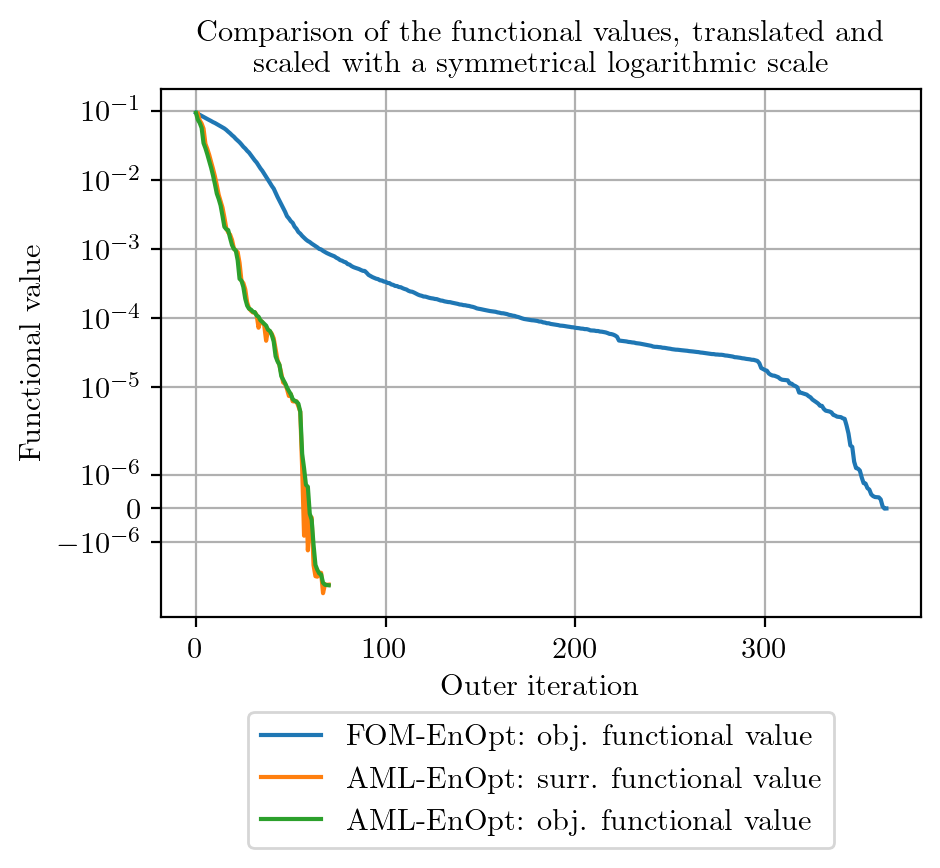
\includegraphics{Plots/functionalValueCompSymlogNT50.png}
\caption{\label{FOMAMLEnOptFuncValCompNT50}The FOM objective functional values obtained during the outer iterations of both EnOpt algorithms and the surrogate functional values obtained during the outer iterations of the AML-EnOpt algorithm with $50$ time steps at the top. The plot at the bottom shows these values, translated by the objective functional value of the FOM-EnOpt output and scaled with a symmetrical logarithmic scale as in Figure \ref{FOMAMLEnOptFuncValComp}.}
\end{figure}

\begin{table}
%\footnotesize
\caption{\label{FOMAMLEnOptParametersNT50}Parameters used in the FOM-EnOpt and AML-EnOpt algorithms with $50$ time steps}
\centering
\begin{tabular}{ll}
\hline
Parameter & Value\\
\hline
Elements of the initial constant control vector $\mathbf{q}_0$ & -40\\
Initial step size $\beta_1$ & $1$\\
Initial covariance matrix adaption step size $\beta_2$ & $0.001$\\
Initial trust-region step size $\delta_\mathrm{init}$ & $100$\\
Step size contraction $r$ & $0.5$\\
Maximum step size trials $\nu^*$ & $10$\\
Maximum (outer/ inner) iterations $k^*, k^*_o, k^*_i$ & $1000$\\
Maximum trust-region iterations $k^*_\mathrm{TR}$ & $5$\\
Initial control variance $\sigma^2_1$ & $0.01$\\
Constant correlation factor $\rho$ & $0.99$\\
Sample size $N$ & $100$\\
FOM-EnOpt $\varepsilon$ & $10^{-14}$\\
Adaptive-ML-EnOpt inner iteration $\varepsilon_i$ & $10^{-14}$\\
Adaptive-ML-EnOpt outer iteration $\varepsilon_o$ & $10^{-14}$\\
%& $$\\
\hline
\end{tabular}
\end{table}

\begin{figure}
\centering
%\textbf{Your title}\par\medskip
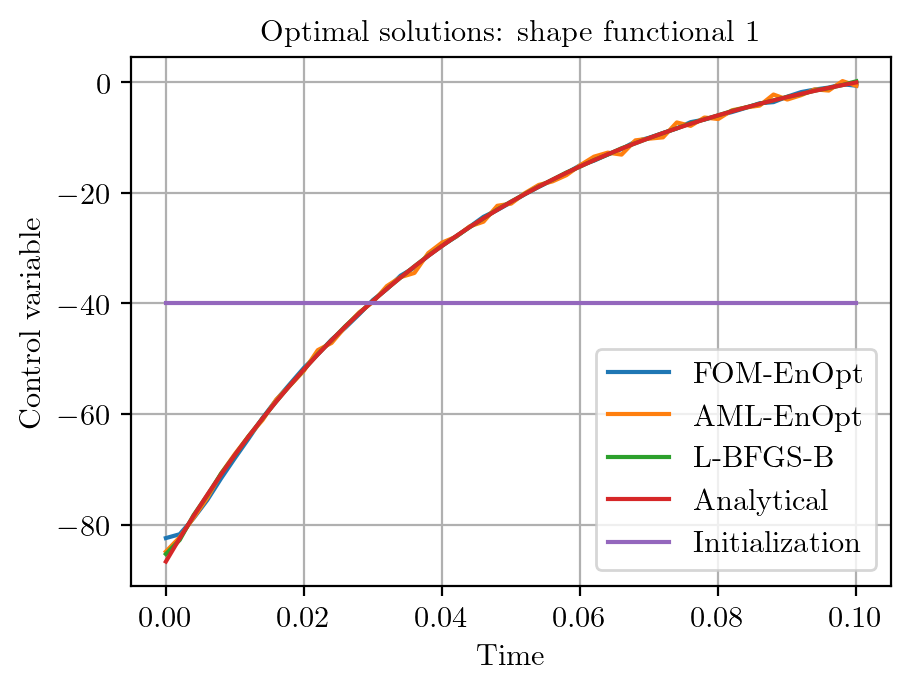
\includegraphics{Plots/solutionsNT50.png}
\caption{\label{solutionsNT50Plot}Comparison of the initial value of the iterate and the optimal solutions obtained from the FOM-EnOpt, AML-EnOpt and L-BFGS-B algorithms for $50$ time steps}
\end{figure}

\begin{figure}
\centering
%\textbf{Your title}\par\medskip
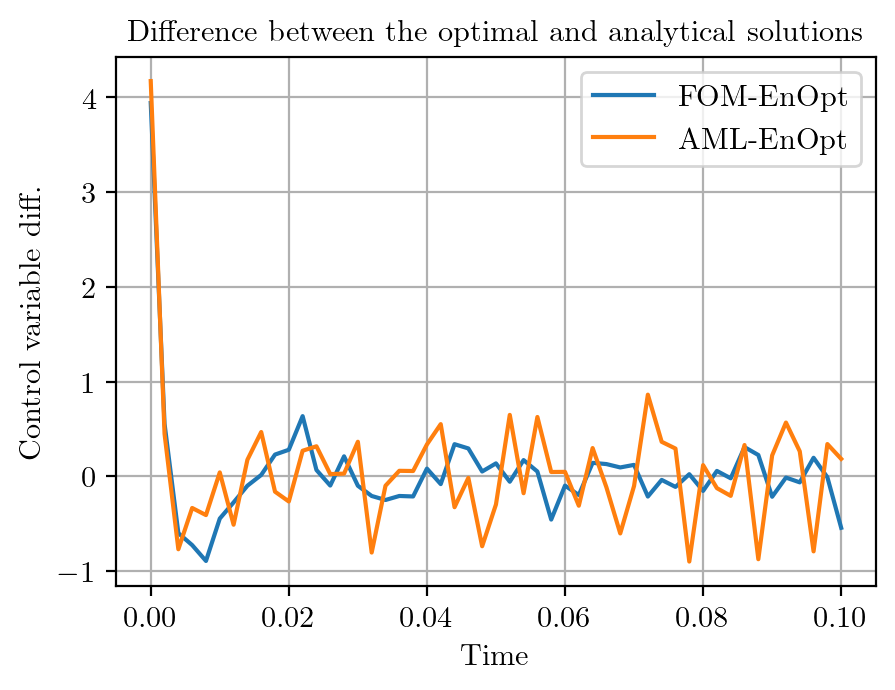
\includegraphics{Plots/solutionsDifferNT50.png}
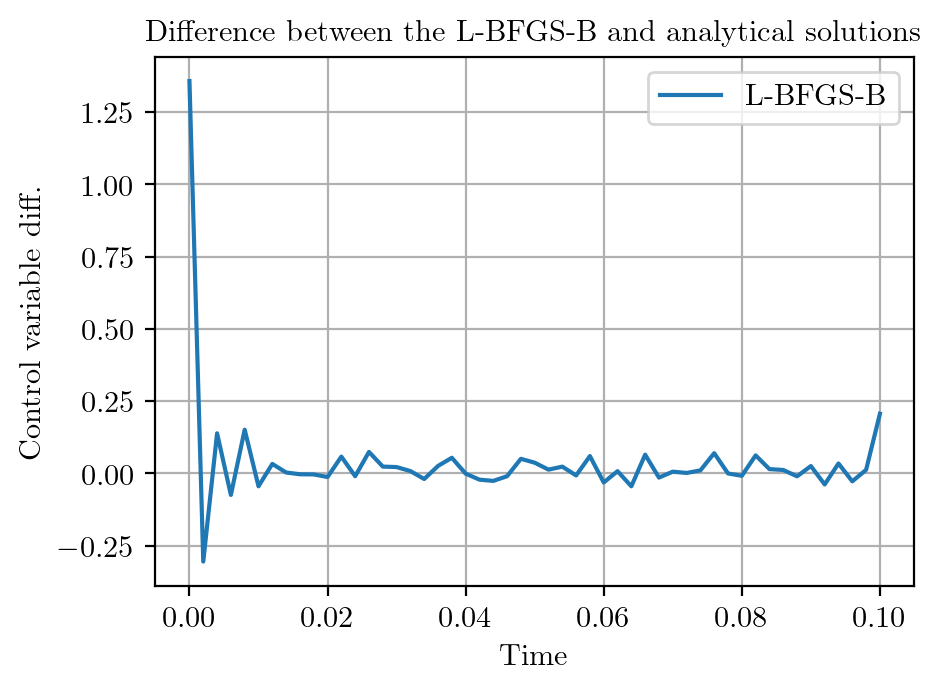
\includegraphics{Plots/solutionsDifferLBFGSBAnalyticalNT50.png}
\caption{\label{solutionsDifferNT50}The differences between the EnOpt solutions and the analytical solution at the top, and the difference between the L-BFGS-B and analytical solution at the bottom for $50$ time steps}
\end{figure}

\begin{figure}
\centering
%\textbf{Your title}\par\medskip
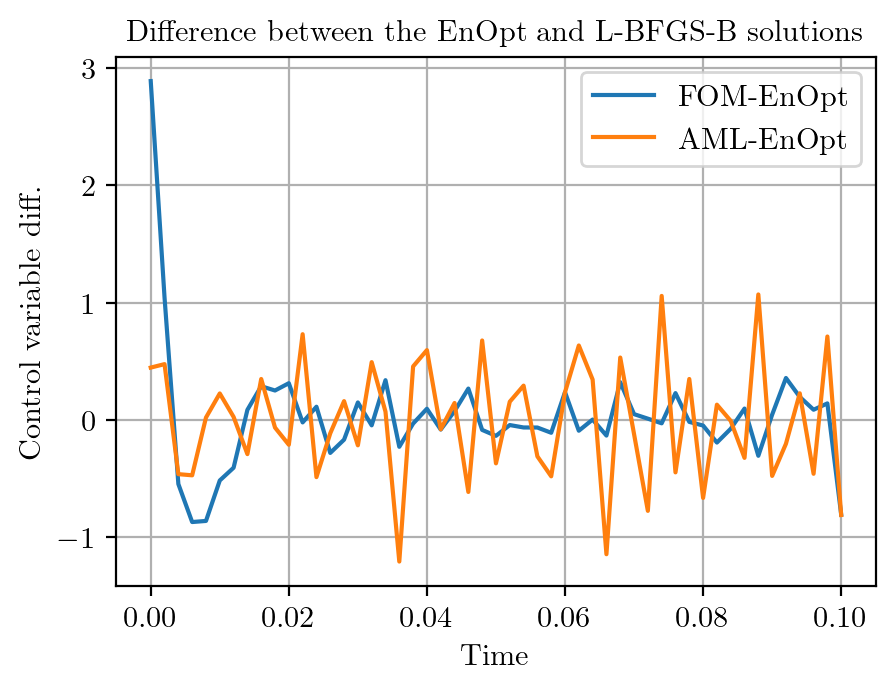
\includegraphics{Plots/solutionsDifferLBFGSBNT50.png}
\caption{\label{solutionsDifferLBFGSBNT50}The differences between the EnOpt solutions and the L-BFGS-B solution for $50$ time steps}
\end{figure}